\chapter{Cosmic Rays and Neutrinos}
\label{ch:cr}
\begin{flushright}
\textit{\\We sit in the mud, my friend, and reach for the stars $\sim$ Ivan Turgenev\\}\end{flushright}

%\url{https://indico.cern.ch/event/719824/contributions/2972435/attachments/1745570/2825844/ISAPP2018_CERN_parizot.pdf} NALEZEN

\noindent Cosmic rays, contrary to their name, almost exclusively exist of particles with a finite rest mass. The term \textit{rays} was historically attributed to these particles as they were thought to be mostly electromagnetic radiation. They are particles coming from outer space, impinging on our atmosphere and producing other particles and large showers of electromagnetic radiation.
The interest in cosmic rays within the field of modern particle physics is clear: many new particles were discovered from the interactions at energies that were higher than most experiments could reach. Positrons, muons, pions, and kaons were first discovered in cosmic ray experiments in the 1930s and 1940s. Today, high-energy cosmic ray interactions are still of interest as the highest energies of these particles go beyond what is feasible even at the most powerful accelerators such as the LHC.

Complementary to cosmic ray experiments is the field of neutrino astronomy as neutrinos are expected to be produced together with cosmic rays, near the source or close to Earth. This makes neutrino astronomy an interesting and possibly powerful part of modern day astronomy. This chapter serves as an overview of the origin of cosmic rays and neutrinos with their properties. Both produce particles that are visible in neutrino telescopes such as the IceCube experiment and are important backgrounds in this analysis. For a more exhaustive description of cosmic rays I refer the reader to Ref. \cite{Gaisser:2016uoy}.

\section{Cosmic rays}
\subsection{Discovery of cosmic rays}
With the use of electrometers, the Austrian physicist Victor Hess performed several ground-breaking balloon flight experiments in 1912 to prove that the amount of ionizing radiation increases with altitude \cite{hessnobel:1936}. This was in strong contradiction with the widespread belief that ionizing radiation on Earth's surface mostly originates from radioactive substances in its crust. Hess concluded that extremely penetrating radiation existed. He described this radiation to be coming from space that enters Earth's atmosphere.
Hess later ruled out the possibility that cosmic rays originate from the Sun as his observations showed no particular difference in night and day and during solar eclipses. In the late 1920s, first evidence was found that cosmic rays were charged due to a variation of their intensity with latitude, which indicated that they were deflected by the geomagnetic field \cite{clay:1927a}.

Hess's ideas proved to be correct, but it was wrongfully attributed to electromagnetic radiation by Robert Millikan in the 1920s \cite{PhysRev.32.533}. 

\subsection{What are cosmic rays?}
\label{subsec:whatarecosmicrays}
Cosmic rays are, almost exclusively, nuclei that are stripped of their electrons, making them electrically charged, heavy particles. Around 90\% of the particles are ionized hydrogen atoms or protons; 9\% are alpha particles and 1\% are nuclei of heavier elements. A much smaller fraction of incoming particles are electrons, positrons and antiprotons.

\begin{figure}
\centering
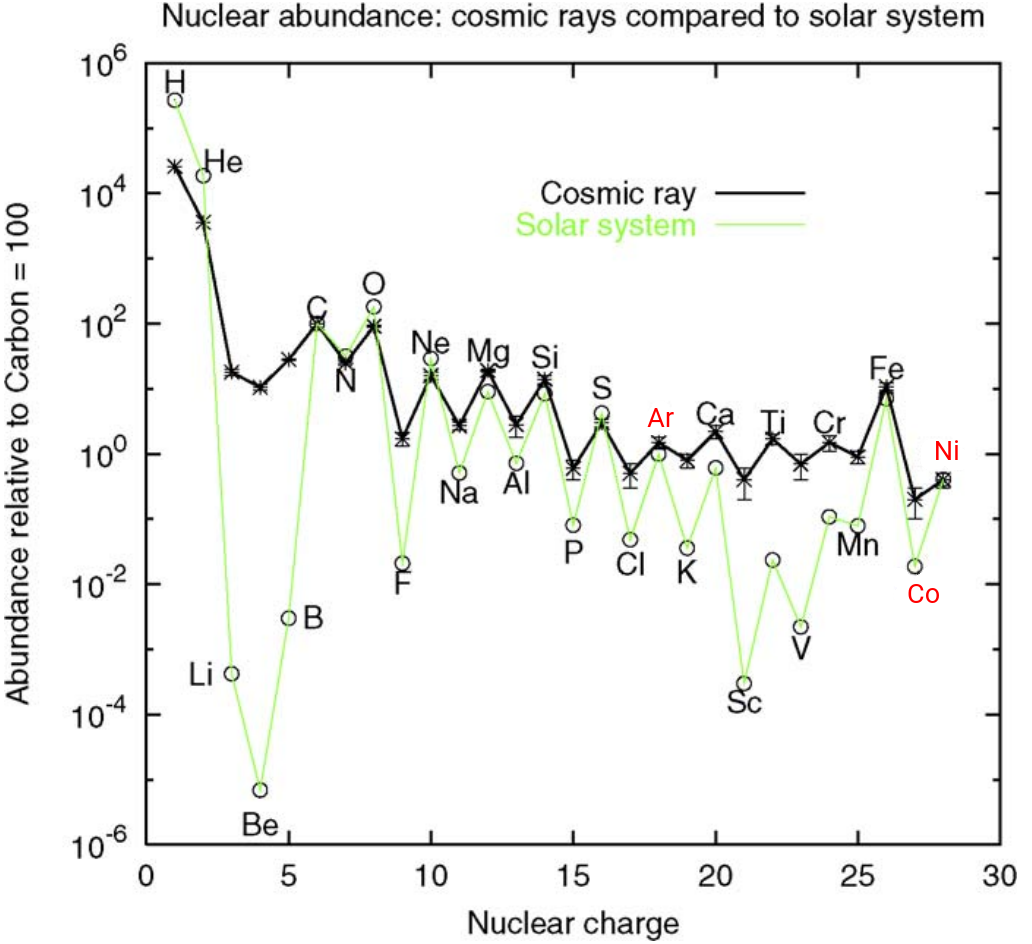
\includegraphics[width=0.7\textwidth]{./chapter3/img/relativeabundanceGaisser.png}
\caption{The cosmic ray elemental abundances with energy $<100$ TeV  measured on Earth compared to the solar system abundances, all relative to ${}^{6}\textrm{C} = 10^2$. Figure from Ref. \cite{GAISSER200698}, with minor corrections in red.}
\label{fig:relabundance}
\end{figure}

There is a striking resemblance between the relative abundance of cosmic rays and elements in the solar system as seen in Figure \ref{fig:relabundance}. There are, however, two important differences between cosmic rays and elements from our solar system. Firstly, the two groups of elements Li, Be, B and Sc, Ti, V, Cr, Mn are many orders of magnitude more abundant in cosmic rays than in the solar system. More massive cosmic rays (mainly C, O and Fe) can produce these nuclei in the process of \textit{spallation}; they are produced by collisions of cosmic rays with the interstellar medium. Therefore, these nuclei are sometimes referred to as \textit{secondary nuclei}. Spallation effects in our solar system are orders of magnitude lower compared to cosmic rays, explaining the difference we see in the relative abundance of these two groups.
The second difference is that nuclei with an atomic number $Z>1$ are much more abundant with respect to hydrogen in cosmic rays. This phenomenon is not yet well understood but might be attributed to the difficulty to ionize hydrogen, necessary for acceleration processes.

The flux of cosmic rays seen on Earth is expressed in units of $\left[\textrm{m}^{-2} \textrm{s}^{-1} \textrm{sr}^{-1}\right]$. We can see in Figure \ref{fig:spectrumCR} that the cosmic ray flux follows a power law energy spectrum

\begin{equation}
\label{eq:spectrum}
dN \varpropto E^{\gamma} dE,
\end{equation} 
where $\gamma$ is called the \textit{spectral index}. Because of the steepness of the spectrum, it is often multiplied by a higher power of energy as can be seen in Figure \ref{fig:spectrumCR}\footnote{The broad range in both energy and flux, visible in Figure \ref{fig:spectrumCR}, should convince the reader that many types of detectors are necessary to study the behavior of cosmic rays. Low-energy particles are abundant and high-energy particles are much more rare. Both the energy and the incoming flux will determine the type and size of the detector.}.

\begin{figure}
\centering
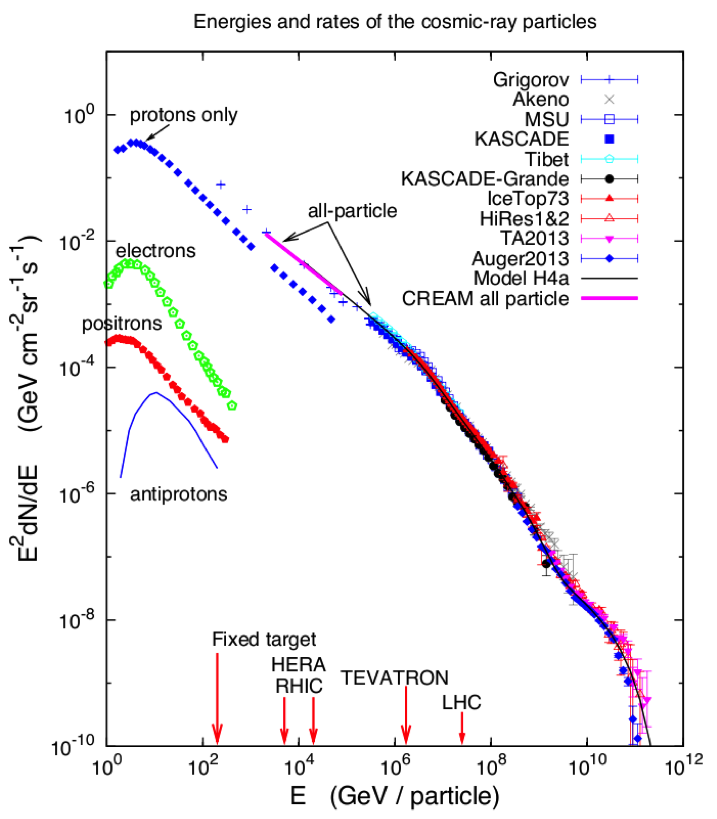
\includegraphics[width = 0.7\textwidth]{chapter3/img/spectrumCR.png}
\caption{Spectrum of cosmic rays at Earth. The all-particle spectrum measured by different experiments is plotted together with the proton-only spectrum. Subdominant contributions to the total flux from electrons, positrons and antiprotons as measured by the PAMELA experiment are also shown. The primary particle energies are compared to accelerator experiments by showing what energy the primary particle should have to reach a similar center-of-mass energy compared to these accelerators, see Eq. \ref{eq:mmax}. Figure from Ref. \cite{Blasi:2013rva}.}
\label{fig:spectrumCR}
\end{figure}

We can divide the global spectrum in four regions. \underline{Between 10 GeV and 1 PeV} the differential spectral index is around -2.7. \underline{From 10 PeV to 1 EeV} it's around -3.1. Below 10 GeV, there is a strong suppression of cosmic rays due to an effect called \textit{solar modulation}\footnote{In the solar system, a stream of charged particles (electrons, protons and alpha particles) is released from the Sun, creating a magnetic field. Cosmic rays coming into the solar system interact with these particles and magnetic field where the influence is greatest on particles with the lowest energies.}. \underline{Above 10 EeV}, the spectrum again flattens to an index around -2.6 and an apparent cutoff region is present at  \underline{around $10^{20}$ eV}. The transition of this first to second region at around 3 PeV is referred to as the \textit{knee}. The second to third region transition is called the \textit{ankle}. It might be possible to describe the full cosmic-ray spectrum with sources within our galaxy. However, a more generally accepted theory is that the knee in the spectrum originates from the end of a population of particles that are accelerated within our Milky Way \cite{Gaisser:2013bla}. Around 100 PeV is the \textit{second knee}, believed to be a feature of the iron drop-off (see Section \ref{subsubsec:galactic}).

The origin of cosmic rays has been a topic of discussion for many years. We now know that most particles originate from sources in the local galaxy, having spent on average $10^7$ years in diffusive motion in the interstellar medium \cite{Gaisser:2013bla}. This is consistent with the similar features of the relative abundances of cosmic rays and elements from our solar system. However, there is no general consensus about the origin of the cosmic rays with energies above 3 EeV. In the following, the above-mentioned energy regions are discussed in more detail.

%\subsubsection{Solar modulation}
%In the solar system, a stream of charged particles is released from the Sun. This stream is mostly made up of electrons, protons and alpha particles with kinetic energies ranging between 0.5 and 10 keV. Within this solar wind plasma, there is a magnetic field. Cosmic rays coming into the solar system interact with these particles and magnetic field. The influence is greatest on particles with the lowest energies. This effect is called \textit{solar modulation}. In effect, we see a strong suppression of cosmic rays at energies of 10 GeV and below.



\subsubsection{Galactic component}
\label{subsubsec:galactic}
It is believed that low-energy cosmic rays have a galactic origin. The most probable acceleration mechanism is by shocks driven by expanding supernova remnants (SNRs) \cite{0034-4885-64-4-201}. This is supported by observations of a lower gamma-ray emissivity from $\pi^0$ decay from Magellanic Clouds compared to the Milky-Way \cite{Fermi-LAT:2010fcp} and the detection of a typical $\pi^0$-decay in the $\gamma$-spectrum from SNRs \cite{Ackermann:2013wqa}. 

With their approximate energy density of around 0.5 eV/cm$^3$ in our local galaxy, the cosmic ray energy density results into a total power of around

\begin{equation}
L_{CR} = 7 \times 10^{40} \textrm{ erg/s},
\end{equation}
where erg is a unit often used in astronomy\footnote{1 erg = $10^{-7}$ J.}. If one assumes a supernova explosion rate of around one per every 30 years, then the total power output of type II supernovae with a mass output of around ten times the mass of the Sun at a velocity close to $5 \times 10^{8}$ cm/s would result in a power of

\begin{equation}
L_{SN} \backsim 3 \times 10^{42} \textrm{ erg/s}.
\end{equation}
These numbers are not set in stone and hold large uncertainties, but it shows that with an acceleration efficiency on the order of a couple of percent, supernova explosions could be a prominent source of energetic cosmic rays, if not the dominant one.

It is still unclear if the galactic component is solely due to SNRs or if other possible sources, such as pulsars, have a measurable contribution.

From the ratio of primary to secondary nuclei, it can be inferred that cosmic rays travel distances thousands of times greater than the thickness of the disk of the galaxy. There is also an apparent decrease in the amount of matter that is traversed by cosmic rays with higher energies than with lower. Higher-energy cosmic rays seem to spend less time in the galaxy than lower-energy ones which suggests that cosmic rays are accelerated before most propagation occurs \cite{Gaisser:2016uoy}.

The way the cosmic ray spectrum is fit is not set in stone. Here I will use the convention used by Gaisser, Stanev and Tilav described in Ref. \cite{Gaisser:2013bla}: the spectrum is subdivided in three populations. The first population corresponds to the particles that are primarily accelerated by supernova remnants, with the knee signaling the cutoff of this population. The second population is a higher-energy galactic component of unknown origin. The third generation will be described in more detail in Section \ref{subsec:extragalactic}. Analogously to Ref. \cite{Gaisser:2013bla}, we assume that the \textit{magnetic rigidity}, $R$, is an appropriate variable for interpreting changes in the spectrum due to propagation and acceleration in magnetic fields. The rigidity is defined as

\begin{equation}
R = \frac{pc}{Ze},
\end{equation}
where $Ze$ is the charge of a nucleus of total energy $E_{tot} = pc$. This assumption follows from the consideration that cosmic rays are accelerated via moving magnetic fields. 

The magnetic rigidity relates to the gyroradius of a particle, $r_g$, in a given magnetic field $B$ as

\begin{equation}
\label{eq:gyro}
r_g = \frac{R}{B}.
\end{equation}
If there is a characteristic rigidity, $R_e$, above which a particular acceleration process reaches a limit, then the feature will show up in total energy first for protons, then for helium and so forth for heavier nuclei according to

\begin{equation}
E_{tot} = Ze \times R_e.
\end{equation}
This effect is visualized in Figure \ref{fig:fitsgaisser} and indicates that as one population reaches its maximum, the composition becomes heavier. The second knee, reported by KASCADE-Grande \cite{Apel:2011mi} and GAMMA \cite{Garyaka:2008gs} could be explained with an ``iron knee'' bump.

\begin{figure}
\centering
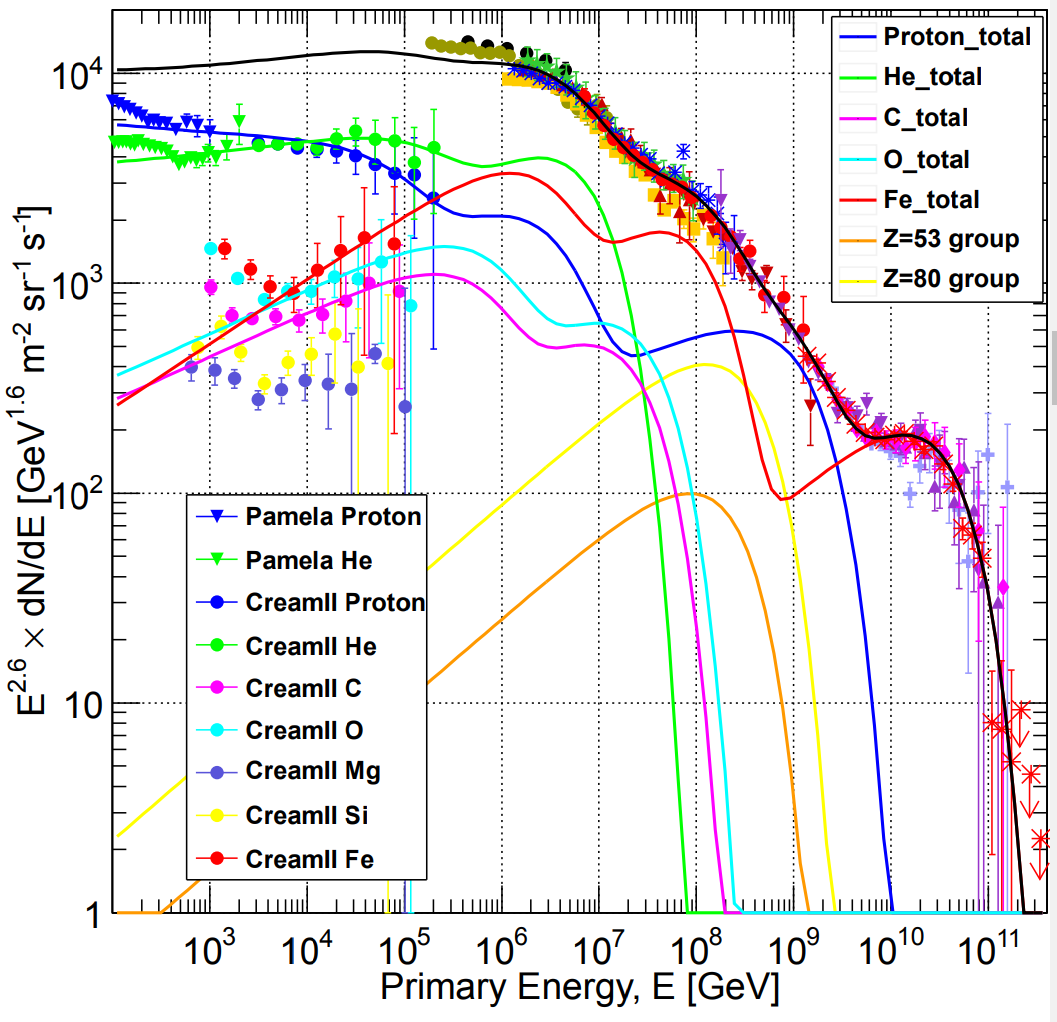
\includegraphics[width=0.48\textwidth]{chapter3/img/fit1gaisser.png}
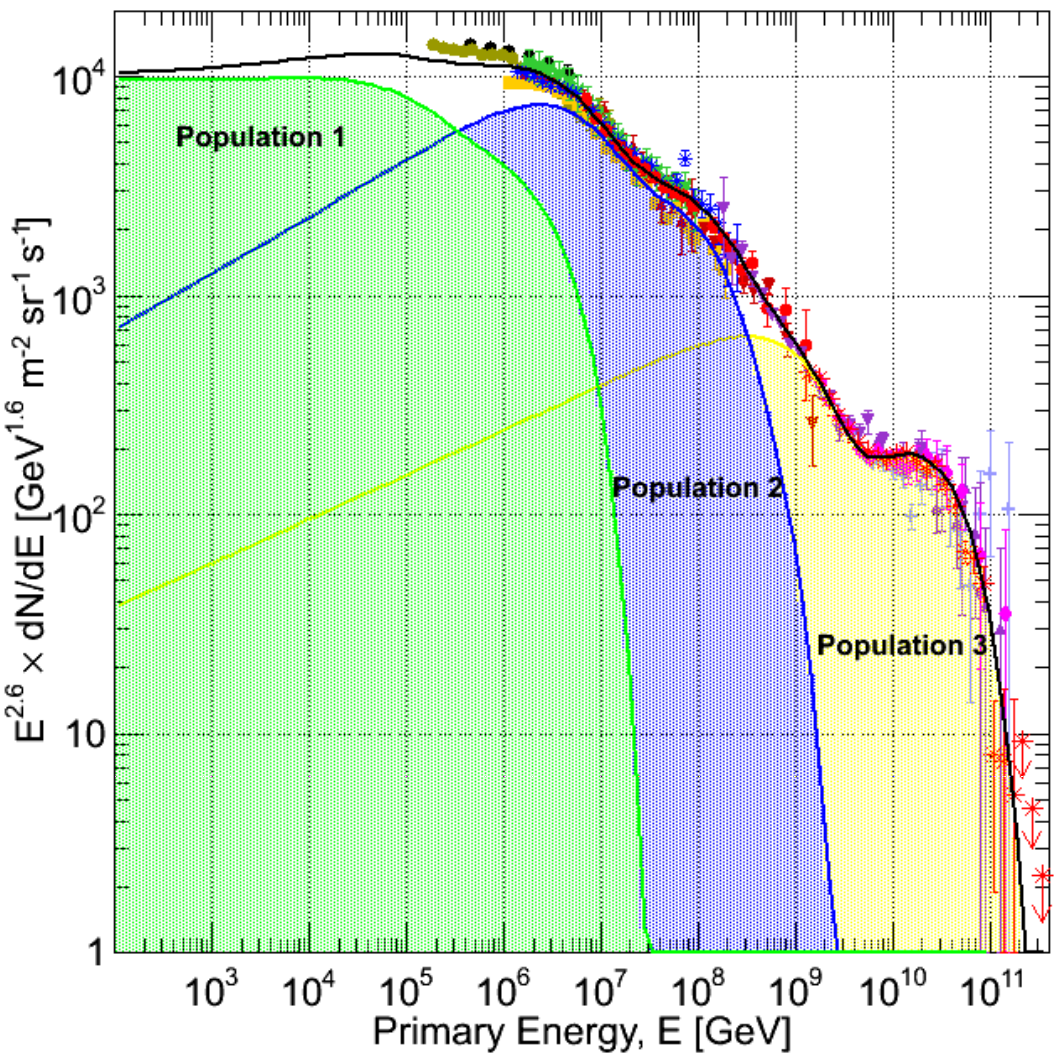
\includegraphics[width=0.48\textwidth]{chapter3/img/fit2gaisser.png}
\caption{Overview of the categorization of the cosmic-ray spectrum as done in Ref. \cite{Gaisser:2013bla}. The individual components are shown on the left, and the total contribution of the three proposed populations are shown on the right.}
\label{fig:fitsgaisser}
\end{figure}

%A schematic picture of our home galaxy, the Milky Way, is shown in Figure 1.2. Most stars are concentrated in the galactic disc of height h $\approx$ 300 pc in the form of spiral arms. The disc is filled with warm atomic gas that consists to 90\% of H and to 10\% of He and has an average density n approx 1/cm3. It contains also an ordered magnetic field with strength B approx 3microG. The energy when the Larmor radius
\subsubsection{Extragalactic component}
\label{subsec:extragalactic}
Very-high-energy cosmic rays are almost certainly from extragalactic origin and result in a flux at the highest energies that is exceedingly small. The number of events at energies above 5 EeV is around one per square kilometer per century. There are only two experiments in the world capable of detecting the highest-energy cosmic rays in a statistically meaningful way: Telescope Array, located in the Northern Hemisphere (instrumented area of $\approx$700 km$^2$) and the Pierre Auger Observatory in the Southern Hemisphere (instrumented area of $\approx$3000 km$^2$).

Both experiments see a suppression of the flux above $6 \times 10^{19}$ eV as seen in Figure \ref{fig:ankle}. The cutoff is consistent with the expected Greisen-Zatsepin-Kuzmin (GZK) effect \cite{Greisen:1966jv,Zatsepin:1966jv} where cosmic rays interact with the cosmic microwave background radiation (CMB)

\begin{equation}
\gamma_{\textrm{CMB}} + p \rightarrow \Delta^+ \rightarrow p + \pi^0
\end{equation} 
or

\begin{equation}
\gamma_{\textrm{CMB}} + p \rightarrow \Delta^+ \rightarrow n + \pi^+.
\end{equation}
The Pierre Auger experiment reported to see higher compositions at the highest energies \cite{icrc2017:pa}. If the particle is a nucleus with $A$ nucleons, then the GZK limit applies to its nucleons, which carry only a fraction $1/A$ of the total energy. For iron nuclei this would for example result in a limit of $2.8 \times 10^{21}$ eV. In contrast, the TA experiment interpreted their data as implying a light primary composition (mainly p and He) at the highest energies. Both experiments use a different interpretations for crucial quantities of these measurements and a thorough joint analysis conducted by both experiments states that, at the current level of statistics and understanding of systematics, both data sets are compatible with being drawn from the same parent distribution \cite{PDG2018url}.

It is also possible that the cutoff corresponds to the ``end-of-steam'' for cosmic accelerators \cite{Allard:2008gj} and that the differences in PA and TA lies at a fundamental difference between northern and southern skies.\\

\begin{figure}
\centering
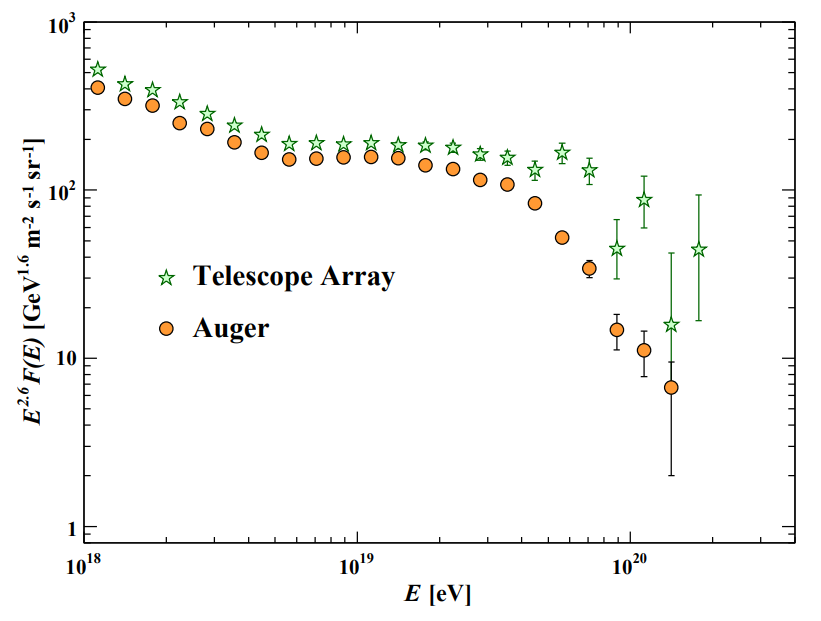
\includegraphics[width=0.6\textwidth]{chapter3/img/ankle.png}
\caption{Expanded view of the highest energy portion of the cosmic-ray spectrum from data of the Telescope Array and the Pierre Auger Observatory \cite{PDG2018url}.}
\label{fig:ankle}
\end{figure}

\noindent The exact origin of Ultra High Energy Cosmic Rays (UHECR) is uncertain. We will see in Section \ref{para:maxenergy} that the maximum energy from shock acceleration by a supernova remnant is insufficient to explain UHECRs. Particles can be accelerated if the trajectory of the particles can be changed and energy can be transferred multiple times. The magnetic fields responsible for the course change of these particles have to be sufficient in magnitude in order for these particles not to escape and go beyond the reach of the source responsible for the acceleration. This limitation is expressed by the gyroradius of the accelerator, $r_L = E/ZeB$ similar to Eq. \ref{eq:gyro}, requiring it to be smaller than the physical radius of the accelerator: $r_L < R$ or $E < ZeBR$.

Even if only qualitative, this relation provides an interesting criterion to identify possible sources of UHECRs by looking at the accelerator related term $BR$. This was done in a classic paper by Hillas \cite{Hillas:1985is}, illustrated in the more recent Figure \ref{fig:hillas}. Accelerators necessary to explain the amount of UHECRs are not populated (enough) in our galaxy, making them more likely to be of extra-galactic origin. Active galactic nuclei, gamma ray bursts, starburst galaxies, and galaxy clusters, which are currently thought to be the sources of UHECRs, are therefore also briefly explained.

\begin{figure}
\centering
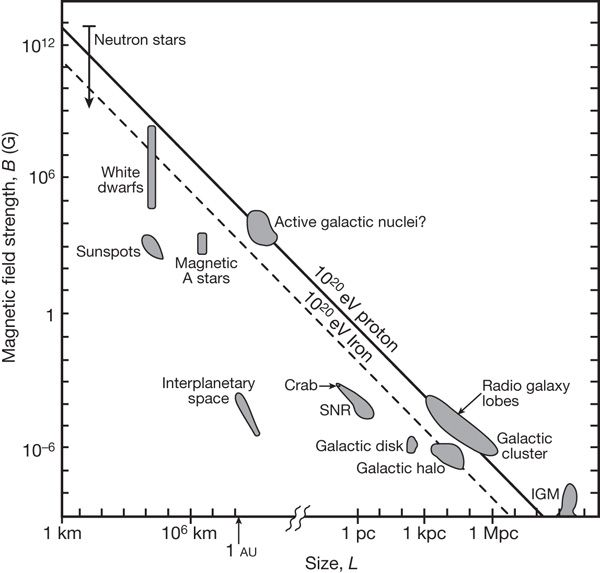
\includegraphics[width = 0.7\textwidth]{chapter3/img/Hillas.jpg}
\caption{The Hillas plot of potential cosmic ray accelerators determines objects according to size and magnetic field. Objects to the left of the diagonal lines cannot accelerate particles to $10^{20}$ eV (proton: solid, iron: broken). Image obtained from Ref. \cite{Bauleo:2009zz}.}
\label{fig:hillas}
\end{figure}

To this date, it has not been proven that these sources all contribute and if they are the sole contributors. There are also more exotic theories on the origin of UHECRs, such as the decay of super-heavy particles \cite{Nagano:2000ve}.



The Pierre Auger Observatory also reported evidence for an anisotropic distribution of the arrival directions of the highest-energy cosmic rays from a direction where the distribution of galaxies is relatively high and does not coincide with the galactic plane \cite{Aab:2017tyv}. These observations, together with our lack of known possible sources within our galaxy for these ultra-high energies, are compelling evidence that these particles have an origin from outside our galaxy. From pion decay, there is also an expected flux from extragalactic neutrinos (more information in Section \ref{subsec:astro}). The flux, spectrum and angular distribution of the excess neutrino signal detected by IceCube between $\approx$50 TeV and $\approx$ 2 PeV are also inconsistent with those expected for Galactic sources \cite{Waxman:2013zda}.\\


%\newline
%To put it simply, understanding cosmic rays and determining their origin can help us answer fundamental questions about the origins of the universe, our galaxy and, more philosophically, ourselves. With the words of Carl Sagan:

%\begin{center}
%\begin{minipage}[5cm]{0.9\textwidth}
%\textit{``The nitrogen in our DNA, the calcium in our teeth, the iron in our blood, the carbon in our apple pies were made in the interiors of collapsing stars. We are made of starstuff.''}
%\end{minipage}
%\end{center}

\subsection{Acceleration mechanism}
How cosmic rays get their signature slope and the intricate details in the energy spectrum have been under discussion for multiple decades. To this date, there is no clear detailed picture how these particles are accelerated. It is beyond the scope of this work to give a comprehensive overview of all possible acceleration mechanisms or possible sources. Most calculations are left out and for a more detailed discussion, the reader is referred to specialized books or the references in the text.\\
\newline
The acceleration of the particles can be subdivided into two questions. First, where are the particles accelerated? Does it happen on large scales, cosmological distances in galaxies or near specific sources? Secondly, how are these particles exactly accelerated? What is the driving mechanism? Since primary cosmic rays are all electromagnetically charged particles, these mechanisms should clearly be sought for in places where electric and/or magnetic fields play a dominant role. Below, a summary of the possible sources is given.




\subsubsection{Supernova (remnants)}
\label{subsubsec:supernovae}
Supernovae can be broadly subdivided in two categories: type I and type II. Type I supernova explosions happen in binary star systems. In those systems, one of the two stars is a carbon-oxygen white dwarf that accretes matter from the second star. When the total mass of the white dwarf reaches the Chandrasekhar limit of around 1.44 solar masses, it cannot longer hold itself under the gravitational pressure and collapses in on itself. Within seconds, the carbon component in the white dwarf starts nuclear fusion and enough energy is released to produce an explosion brighter than the Sun with a factor of around 5 billion. 
A resulting shock wave can reach up to around 3\% of the speed of light.

Type II supernova explosions differ by being single star systems. When a star reaches the end of its life cycle, the subsequent fusion reactions reach a halt. If the star has enough mass (at least 8 times the mass of the Sun), it is possible for the inner core to again reach the Chandrasekhar limit and collapse in on itself due to the lack of \textit{electron degeneracy}. Without the outward pressure of nuclear fusion reactions and the support of the core, the outer layers of the star collapse under the gravitational pressure. The compression of the electrons and protons into neutrons results in a very hot, dense, neutron core. The velocity of the inward falling layers can reach a staggering 23\% of the speed of light and recoil when hitting the remaining core. The outward going shock wave hits the remaining outer layers forming the supernova explosion\footnote{To get a better feeling of how extraordinary these events really are, I'd like to illustrate what it would be like if one could be close to a supernova event. From Figure \ref{fig:neutrinospectrumall}, one can calculate that the number of solar neutrinos going through our hand per second is around \textit{one trillion}. Yet they are so weakly interaction that, on average, only one will interact with an atom in our body every few years. Supernova explosions are vast, releasing around $10^{57}$ neutrinos. This number is large enough that even if an observer is a distance of 2.3 AU away from the event, he would still receive a fatal radiation dose of \textit{neutrinos alone}. Another example: looking at a supernova at a distance of 1 AU is $10^9$ times brighter than detonating a hydrogen bomb pressed against your eyeball.}. This violent core collapse is an additional neutrino production mechanism.

Because of their brightness, supernovae within our galaxy can be seen with the naked eye (provided they are not obscured). The last recorded supernova from our galaxy was by Kepler in 1604 but the earliest recordings go back to 185 AD by Chinese astronomers\footnote{From observations of other galaxies, supernovae are expected to occur, on average, once every thirty years. Not all of these will be visible to the naked eye, but would almost certainly be observable with modern astronomical telescopes.}.
\begin{figure}
\centering
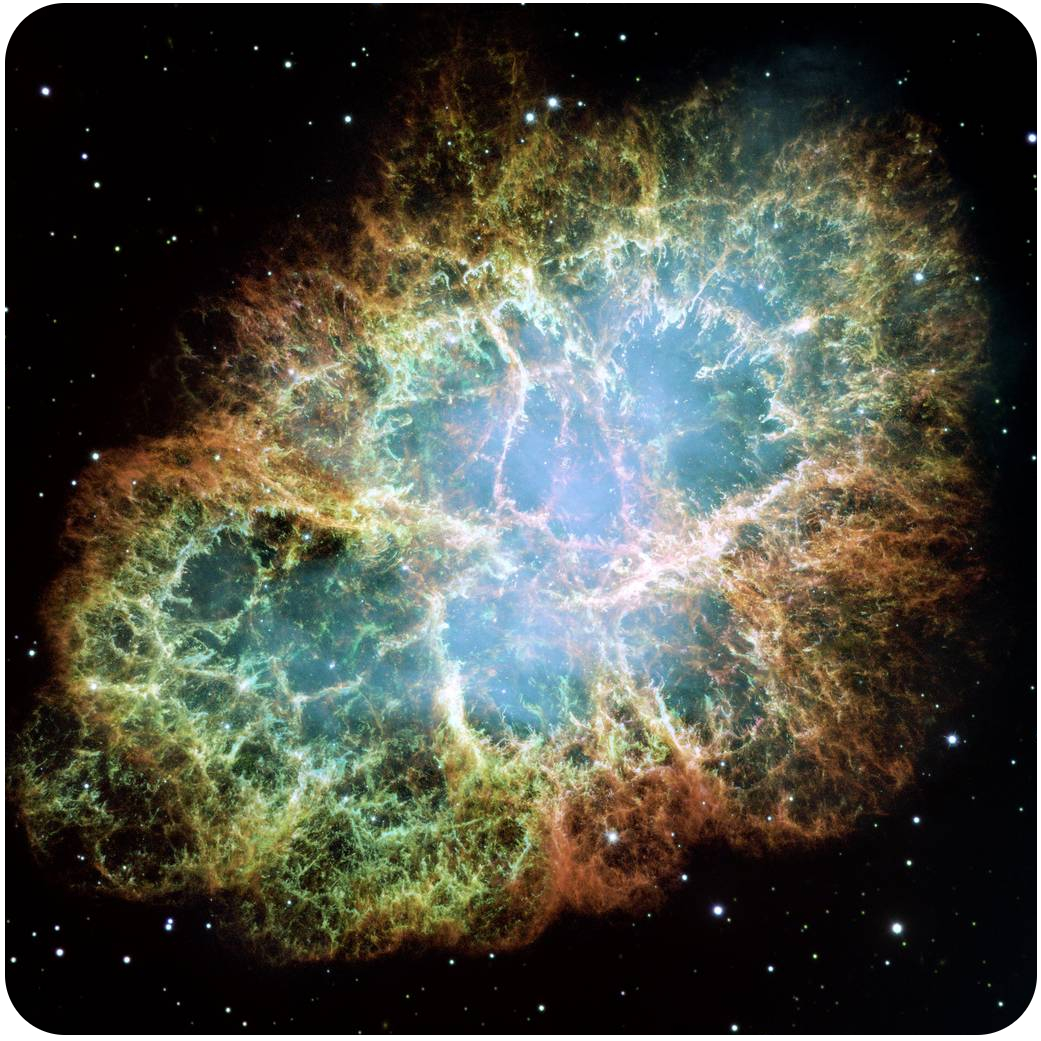
\includegraphics[width=0.48\textwidth,height=7.7cm]{chapter3/img/crabnebula_rounded.jpg}
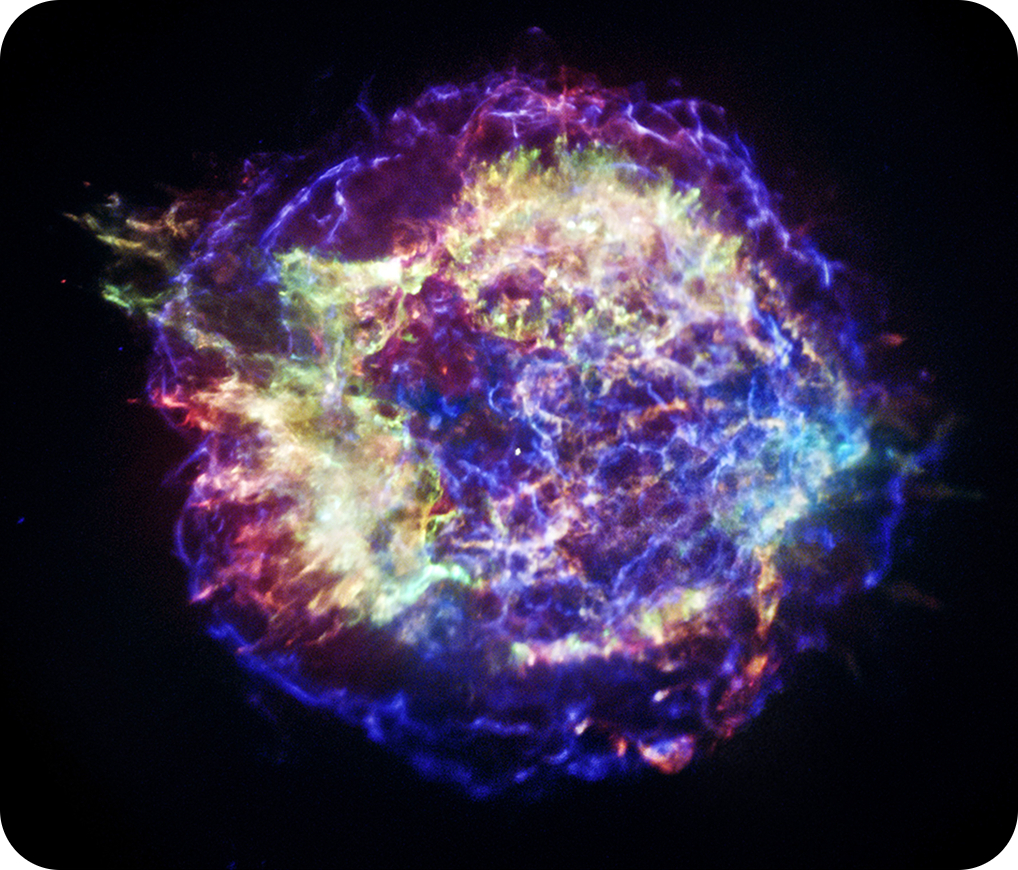
\includegraphics[width=0.51\textwidth,height=7.7cm]{chapter3/img/casa_rounded_resized.jpg}
\caption{\textit{Left}: the Crab Nebula is a supernova remnant approximately one thousand years old. The supernova was noted by Chinese astronomers in the year 1054 AD. \textit{Right}: Chandra X-ray observatory picture of the Cassiopeia A supernova remnant (pictures from NASA).}
\label{fig:supernova}
\end{figure}
\newline
The question remains how supernovae can serve as cosmic ray accelerators. In 1949, Fermi proposed a mechanism where particles can gain energy by collisions with moving interstellar ionized gas clouds. Only later, it was realized that a large, plane shock front moving with a certain velocity is able to accelerate charged particles much more efficiently. This first mechanism results in an energy transfer proportional to the squared velocity of the cloud and is thus called \textit{second order Fermi acceleration}. Shock front acceleration energy transfer is proportional to the velocity and is called \textit{first order Fermi acceleration}. Supernova remnants provide an explanation for the origin of these shock fronts.

\paragraph{First- and second-order Fermi acceleration}
\label{para:fermiacceleration}

Suppose we have a magnetic cloud in the interstellar medium travelling with a certain velocity $\vec{V}$ and a particle with velocity $\vec{v}$ enters the cloud under an angle $\theta_1$ (see Figure \ref{fig:cloud}). If we assume collisionless scattering (no energy is dissipated from the particle to the cloud) due to the magnetic fields in the cloud, the magnitude of the momentum in the rest frame of the cloud will not change ($E'_1 = E'_2$, where the apostrophe denotes the cloud rest frame). From special relativity we know that:

\begin{figure}[t]
\begin{minipage}{6in}
  \centering
  \raisebox{-0.5\height}{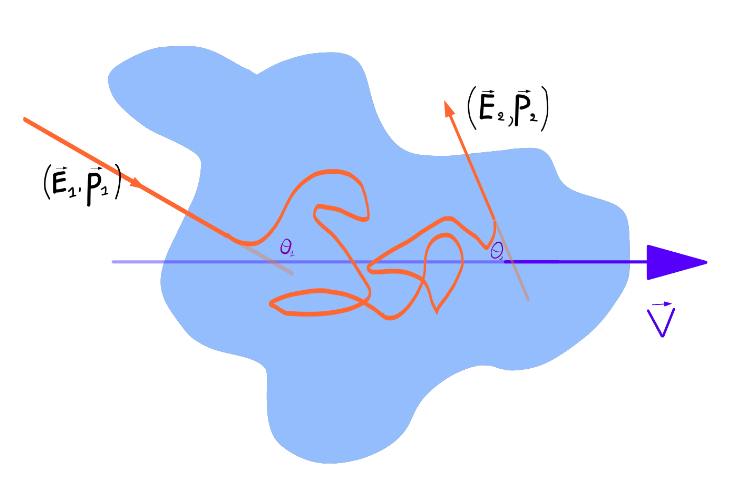
\includegraphics[height=2in]{chapter3/img/cloud_update.png}}
  \hspace*{.1in}
  \raisebox{-0.5\height}{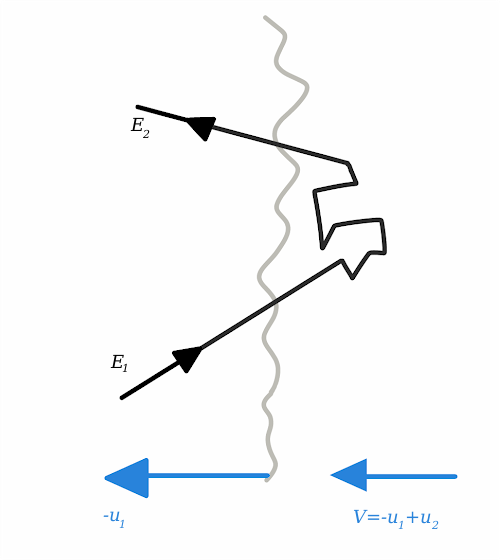
\includegraphics[height=3.1in]{chapter3/img/shock.png}}
\end{minipage}
\caption{\textit{Left}: magnetic cloud showing second-order Fermi acceleration. \textit{Right}: shock waves typically have magnetic inhomogeneities both preceding (downstream) and following them (upstream). If a charged particle travels through the shock wave, it can gain velocity through first-order Fermi acceleration. In the illustration, a particle travels from upstream to downstream and back upstream. At every back and forth movement, the particle effectively gains energy. For a particle with a velocity $u_1$ relative to the shock front, the front seems to come at him with velocity $-u_1$. The downstream medium has a velocity relative to the shock front of $u_2 < u_1$ making it seem coming towards the particle with velocity $u_1-u_2$.}
\stepcounter{figure}%
\label{fig:cloud}
\end{figure}

\begin{equation}
\begin{split}
E'_1 &= \gamma \left(E_1 - p_{1,\parallel} V\right) \\
&= \gamma E_1 \left(1-\beta \cos \theta_1\right),
\end{split}
\end{equation}
with $\beta = V/c$ and $\gamma$ the Lorentz factor. Similarly, and using $E'_1 = E'_2$

\begin{equation}
\begin{split}
E_2 &= \gamma E'_2 \left(1+\beta \cos \theta_2'\right)\\
&=\gamma^2 E_1 \left(1-\beta \cos \theta_1\right) \left( 1 + \beta \cos \theta_2'\right)
\end{split}
\end{equation}
and

\begin{equation}
\frac{\Delta E}{E} = \frac{E_2 -E_1}{E_1} = \frac{1 - 
\beta \cos \theta_1 + \beta \cos \theta_2' - \beta^2 \cos \theta_1 \cos \theta_2'}{1-\beta^2} -1.
\end{equation}
By hypothesis, the escaping particles are isotropic in the cloud frame: $\langle \cos \theta_2' \rangle = 0$. One can show that $\langle \cos \theta_1 \rangle = -\frac{\beta}{3}$ \cite{Gaisser:2016uoy}, leading to

\begin{equation}
\frac{\Delta E}{E} = \frac{4}{3} \frac{\beta^2}{1-\beta^2} \approx \frac{4}{3} \beta^2,
\end{equation}
showing that for molecular clouds, the energy gain is indeed proportional to the square of $\beta$, thus second-order Fermi acceleration.\\
\newline
If a particle is incoming to an expanding shock (see Figure \ref{fig:cloud}), one can prove that $\langle \cos \theta_1\rangle$ is equal to $-2/3$ and $\langle \cos \theta_2'\rangle$ is equal to 2/3, leading to

\begin{equation}
\frac{\Delta E}{E} = \frac{\frac{4}{3}\beta + \frac{13}{9}\beta^2}{1-\beta^2} \approx \frac{4}{3} \beta,
\end{equation}
where $\beta$ is now equal to $u_1 -u_2$, as explained in the caption of Figure \ref{fig:cloud}. We have shown that for shock fronts the energy gain is indeed proportional to $\beta$ for first-order Fermi acceleration. 
%From both the outcome as the discussion it is clear that the energy gain enters through relativistic effects, making an intuitive approach not straightforward.

\paragraph{Power}
\label{para:power}
The energy gain of a ``single collision'' results in a powerlaw spectrum when considering a process in which a test particle increases its energy by an amount proportional to its energy with each encounter. Let us assume $\Delta E = \xi E$, then, after $n$ encounters:

\begin{equation}
E_n = E_0 \left(1+\xi\right)^n,
\end{equation}
where $E_0$ is the energy when the particle first enters the accelerator medium. To reach a certain energy $E'$, the particles must undergo a number of collisions

\begin{equation}
\label{eq:nn}
n(E') = \frac{\ln \left(\frac{E'}{E_0}\right)}{\ln \left(1+\xi \right)}.
\end{equation}
To reach energies of $E'$ or higher, the number of collisions will be proportional to

\begin{equation}
\begin{split}
N(\geq E') \varpropto &\sum^\infty_{m=n} P_{present}(m) = \sum^\infty_{m=n} \left(1-P_{esc} \right)^m\\
&= (1-P_{esc})^n \left((1 - P_{esc}) + (1 - P_{esc})^2 + ...\right) \\
&= \frac{(1-P_{esc})^n}{P_{esc}},
\end{split}
\end{equation}
where $P_{present}$ is the probability of a particle still being present in the accelerator and $P_{esc}$ the probability of the particle to escape per collision. Making use of $a^{\ln b} = e^{\ln a \ln b} = b^{\ln a}$ and inserting Eq. \ref{eq:nn} yields

\begin{equation}
N(\geq E') \varpropto \frac{1}{P_{esc}} \left(\frac{E'}{E_0}\right)^{-\gamma},
\end{equation}
with

\begin{equation}
\gamma = \frac{\ln \left(\frac{1}{1-P_{esc}}\right)}{\ln \left(1 + \xi \right)} \approx \frac{P_{esc}}{\xi}.
\end{equation}
The power law spectrum becomes visible in the derivative of the number of particles in energy

\begin{equation}
\frac{dN}{dE} \backsim E^{-(\gamma + 1)},
\end{equation}
in agreement with Eq. \ref{eq:spectrum} (although $\gamma$ is not the same variable here). Shock wave fronts have an expected $\gamma \approx 1$, giving rise to a different spectrum to what is seen on Earth but which can be explained by propagation from the source to Earth (see \ref{subsec:propagation}). The spectrum from Fermi shock acceleration is thus expected to follow an $E^{-2}$ powerlaw behavior.
%\\
%\newline
%Seems plausible all galactic CRs are accounted for my supernovae. This is supported with the realization that first-order Fermi acceleration naturally produces a spectrum of cosmic rays close to what is observed.

\paragraph{Maximum energy}
\label{para:maxenergy}
The highest energies that particles can be accelerated to can be defined by

\vspace{2mm}
\begin{itemize}
\item the differential energy gain per collision $dE/dt$, and
\item the total time the particle can be accelerated.
\end{itemize}
\vspace{2mm}
\noindent The energy gain is given by
\begin{equation}
\frac{dE}{dt} = \frac{\xi E}{T_{cycle}},
\end{equation}
where $T_{cycle}$ is the characteristic time for one acceleration cycle. $T_{cycle}$ depends on the diffusion coefficients and velocities of the upstream and downstream regions and is set to $T_{cycle} \geq 20 E/(3 u_1 Z e B)$ by Lagage and Cesarsky \cite{Lagage:1983zz} for a strong shock and arguing that the diffusion length, $\lambda_D$, cannot be smaller than the Larmor radius of the particle. Particles with a Larmor radius greater than the irregularities holding a magnetic field are not prone to be heavily influenced by them. Lagage and Cesarsky therefore concluded that

\begin{equation}
E_{max} \leq \frac{3}{20} \frac{u_1}{c} Z e B (u_1 T_{ST}),
\end{equation}
where $T_{ST}$ is the Sedov-Taylor time where particles are less prone to escape and is $\backsim 1000$ years. For $u_1 \backsim 10^9$ cm/s \cite{stanev2010high}  and $B \backsim 3\mu G$ the Lagage and Cesarsky limit reads

\begin{equation}
E_{max} \leq Z \times 2.4 \times 10^{14} \textrm{eV}.
\end{equation}

\subsubsection{Active Galactic Nuclei}
\label{subsubsec:agn}
Active Galactic Nuclei (AGNs) are no stars at the end of their life cycle but active black holes located in the center of galaxies. It is believed that most massive galaxies have supermassive black holes in their centers by the accretion of matter from surrounding large gas clouds \cite{Urry:1995mg,Antonucci:1993sg}. However, this is still under debate. AGN masses in current models range from $10^6$ to $10^{10}$ solar masses \cite{Kazanas:2012sk}.

The efficient conversion of gravitational potential energy to kinetic energy and radiation make AGNs the most luminous persistent sources of electromagnetic radiation in the universe. As such, they serve as very good tools to discover distant objects. The accretion discs heat up due to friction from the inward falling matter and produce light peaking in the ultraviolet waveband. Certain emission lines are also expected due to the radiation from excited cold atomic material. Some accretion discs produce jets, which point opposite to each other. Their direction is defined by either the spin of the black hole, the accretion disc or a combination of both.  The most powerful AGNs are classified as \textit{quasars} and AGNs with a jet pointing toward the Earth are called \textit{blazars}.

\begin{figure}
\centering
%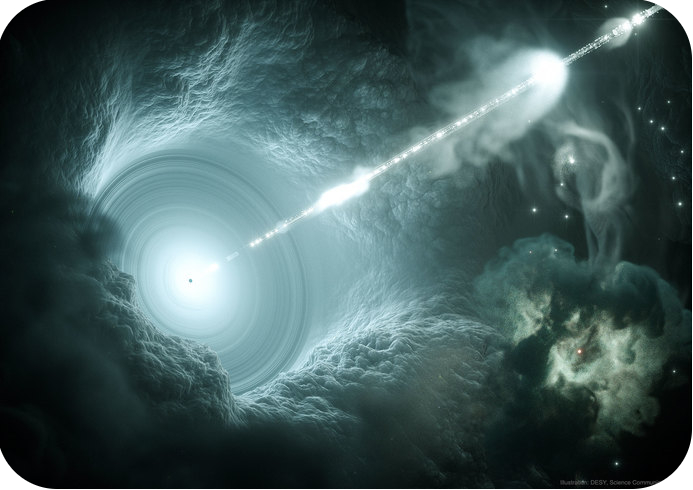
\includegraphics[width=0.49\textwidth]{chapter3/img/quazar_resized_rounded_resized_2.jpg}
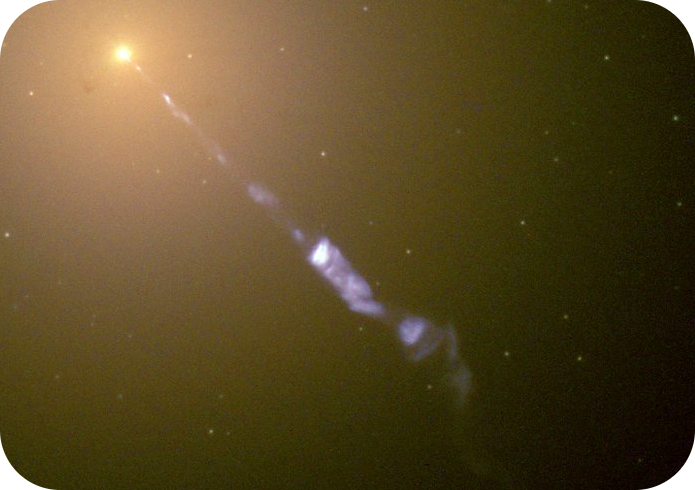
\includegraphics[width=0.55\textwidth]{chapter3/img/jet_crop_rounded.jpg}
\caption{
%\textit{Left}: artist impression of a blazar. Illustration from DESY, Science Communication Lab. \textit{Right}: 
Image from the Hubble telescope where we see a jet streaming out from the center of galaxy M87.}
\end{figure}

Charged particles can have a large magnetic rigidity in AGNs and the relativistic jets could provide the necessary mechanisms to accelerate particles to ultra-high energies. The Pierre Auger collaboration hinted to a correlation of the highest-energy cosmic rays with the positions of nearby active galactic nuclei \cite{Abraham:2007si}.

\subsubsection{Gamma Ray Bursts}
\label{subsubsec:grb}
The most catastrophic deaths of massive stars or mergers of two neutron stars or of a neutron star and a black hole result into Gamma Ray Bursts (GRBs). GRBs are named after the burst of gamma rays that is followed by a longer-lived afterglow of electromagnetic radiation at longer wavelengths. These bursts are the most energetic explosions in the electromagnetic spectrum and occur when a high-mass star collapses to form a neutron star or black hole. A typical burst releases as much energy in a few seconds as the Sun does in its entire 10 billion-year lifetime and temporarily outshines the rest of the galaxy\footnote{GRBs were first discovered in the late 1960s by accident. The Vela satellites had additional gamma ray detectors designed to detect very fast bursts of gamma rays that were expected to be produced by nuclear tests in space \cite{Klebesadel:1973iq}.}. GRBs are isotropically distributed, making them extragalactic in origin \cite{Meegan:1992xg}.

An often used model to explain how charged particles could reach extremely high energies is called the \textit{fireball model}. This internal-external shock model assumes that kinetic energy of an ultra-relativistic flow is dissipated in internal collisions. \\
%When the shock hits the surrounding matter, it is slowed down and gives rise to the signature afterglow \cite{Piran:2004ba}. After an initial progenitor phase (see below), a plasma of photons, electrons, positrons, and baryons develops into the formed jets. In this initial phase, the fireball is radiation-dominated and optically thick for photons, making it invisible in the electromagnetic spectrum. Due to radiative pressure, the fireball expands at relativistic speeds ($\gamma$-factors $>$ 100) to the point that it becomes more and more transparent. If the central engine produces multiple shocks with different velocities, there will be internal shocks, which give rise to the observed burst emission. In this mechanism, the ultra-relativistic matter can transfer its kinetic energy to the acceleration of particles, explaining cosmic ray production. Later shocks of the jets with surrounding matter would explain the signature afterglow seen in GRBs.

\noindent Although there is still much ongoing discussion, GRBs are usually subdivided into two groups: \textit{long gamma ray bursts} ($t_{burst} > 2$ s) and \textit{short gamma ray bursts} ($t_{burst} < 2$ s). Long bursts originate from collapsars: a massive star core-collapse forms a black hole and surrounding matter is pulled into an accretion disk. Short bursts hint to progenitors that are extremely compact, where neutron star-neutron star or neutron star-black hole mergers are the most probable explanation. The recent detection of gravitational waves can provide a significant contribution to the understanding of these sources \cite{TheLIGOScientific:2017qsa,Abbott:2017oio,Abbott:2017gyy,Abbott:2017vtc,Abbott:2016nmj}.

%\begin{figure}
%\centering
%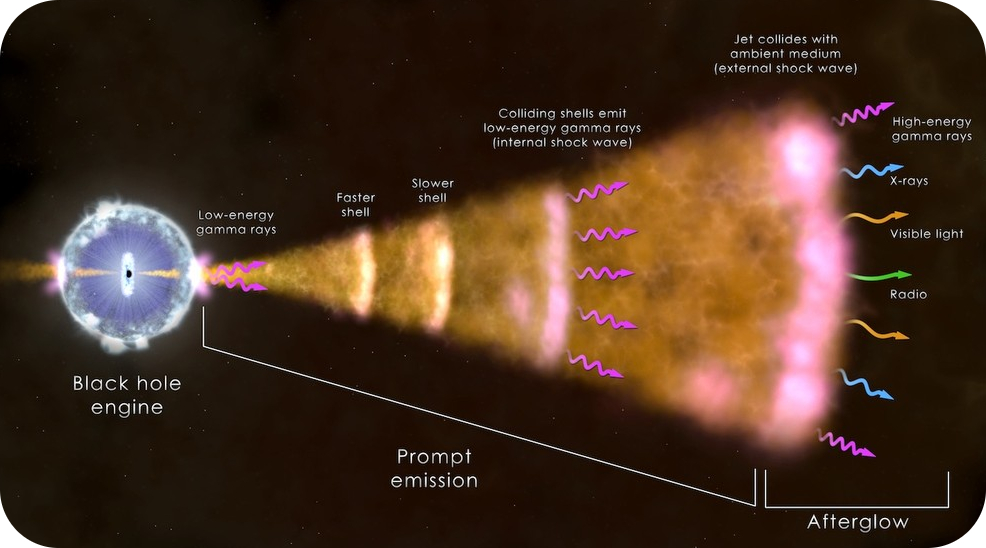
\includegraphics[width=0.6\textwidth]{chapter3/img/fireball_rounded.jpg}
%\caption{Schematic view of the fireball model. In the beginning, the fireball is opaque. After propagation, it becomes transparent, releasing $\gamma$-rays due to high-temperature plasma. Charged particles are accelerated in the shock waves and hit the interstellar medium, emitting optical and X-ray light. Image from NASA Goddard space flight center.}
%\end{figure}

\subsubsection{Starburst galaxies}
Galaxies that undergo an episode of large-scale star formation, are called \textit{starburst galaxies}. Most of these are in the midst of a merger or close encounter with another galaxy. Several experiments have shown their gamma ray emission at several hundred GeV to be two to three orders of magnitude higher than in our own galaxy \cite{Acero:2009nb,Karlsson:2009hd}. Galactic scale winds from the central regions are possible sources for cosmic ray acceleration.

\subsubsection{Galaxy clusters}
When galaxies are bound together by gravity, they are referred to as \textit{galaxy clusters}. They can contain around 100 to 1000 galaxies and have typical mass ranges around $10^{14}-10^{15}$ solar masses. Through merging and accretion of dark matter and baryonic gas, galaxy clusters are expected to generate powerful shock waves on large scales. Shocks with significant velocities could provide the necessary conditions for cosmic ray acceleration \cite{1538-4357-689-2-L105}.

\subsection{Propagation}
\label{subsec:propagation}
After creation, particles also encounter propagation effects on their way to Earth. For example, charged particles can be deviated in magnetic fields close to or far from their source and by the Earth's magnetic field. The particles can interact with expulsed matter from the source soon after their creation. Other possibilities are gas clouds \textcolor{red}{hoe nauwkeurig is dit?}, leading to spallation effects or a loss of energy. The models describing these effects will not be given in this work. However, it is noteworthy to mention that in these models the measured cosmic ray flux becomes much softer than the source flux. The discrepancy between spectral indices around -$2.7$/-$3$ and a theoretical source flux around -$2$ is usually attributed to these propagation effects. For more information, I refer the reader to Ref. \cite{Gaisser:2016uoy}.


\section{Air showers}
\label{sec:airshowers}
When primary cosmic ray particles hit the Earth's atmosphere, they give rise to a large shower of secondary particles. At low- to mid-energy ranges, the abundance of cosmic rays is large enough for these showers to be analyzed with balloon or satellite experiments. As indicated in Section \ref{subsec:whatarecosmicrays}, the flux of high-energy cosmic rays is so small that there is a need for very large-scale detectors, measuring square kilometers in instrumented area.\\
\newline
The interaction length of nuclei with high energies is too small for them to be able to travel as close as a couple of tens of kilometers in height as measured from the ground. They will interact with an atmospheric nucleus and produce secondary particles.
These particles in their turn decay or interact further with the atmosphere and give rise to an \textit{extensive air shower} (EAS) if the production of new particles is large enough. Some of these particles will be stopped, but others are capable of reaching the Earth or even penetrate deep inside it. 
Although air showers are of significant importance in cosmic ray studies, we will only give a brief summary of the most noteworthy features and its main importance for this analysis.
An air shower has three components: the hadronic, muonic, and electromagnetic. An air shower also produces neutrinos. These are discussed in more detail in Section \ref{sec:neutrinos}. The hadronic component can be seen as the core of the shower, consisting of high-energy hadrons. The interactions and subsequent decays of these hadrons fuel the electromagnetic and muonic parts. A schematic overview is given in Figure \ref{fig:airshower}. If the primary particle is a photon, the shower is made up almost exclusively of an electromagnetic component. Because the lateral size of an electromagnetic cascade is caused by multiple scatterings of electrons and positrons, the lateral size of these showers is relatively small (radius around 1 km at sea level for a vertically downgoing 100 TeV photon). In hadronic cascades, on the other hand, the lateral size is caused by the transverse momenta of the secondary particles making these showers much larger (radius around 4 km at sea level for a vertically downgoing 100 TeV proton) \cite{Grupen:2005rx}.

\begin{figure}
\centering
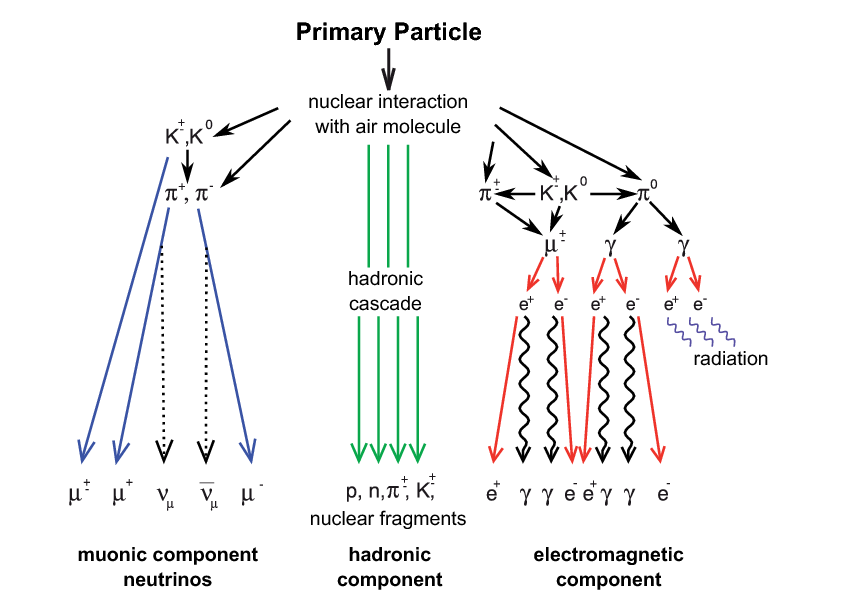
\includegraphics[width=0.8\textwidth]{chapter3/img/airshower.png}
\caption{Schematic view of an extensive air shower with a clear distinction between the three components. Image from the KASKADE collaboration.}
\label{fig:airshower}
\end{figure} 

\subsection{Hadronic component}
When a proton interacts with a nucleus, it interacts with another proton or a neutron and will most often produce charged or neutral pions
\begin{equation}
\begin{split}
p+N &\rightarrow p+N + k\pi^+ + k\pi^- +r\pi^0,\\
p+N &\rightarrow n+N + (k+1)\pi^+ + k\pi^- + r\pi^0,\\
\end{split}
\end{equation}
where $N$ stands for a nucleon of an atmospheric nucleus and $k$ and $r$ are the multiplicities of the produced pions. The extension to heavier nuclei from this is straightforward. On average, one-third of the hadron production will be neutral pions ($k/r \approx 3$), which decay immediately into electromagnetic particles 

\begin{alignat}{2}
\pi^0 &\rightarrow \gamma  +\gamma &&(98.8\%) \textrm{ or}\\
\pi^0 &\rightarrow e^+ + e^- + \gamma \ \ &&(1.17\%).
\end{alignat}
The other two-thirds will be charged particles that have a lot longer lifetime, making them much more probable to interact with air nuclei. After having traveled a distance corresponding to their mean interaction length, charged particles interact again with air nuclei if their energy is large enough. 90\% of these charged particles are new pions and 10\% of the daughter particles are kaons. Pions almost exclusively decay to muons ($\pi^+ \rightarrow \mu^+ + \nu_{\mu}$) and the most dominant kaon decay modes are (similar for $K^-$) \cite{PDG2018url}

\begin{alignat}{2}
K^+ &\rightarrow \pi^+ + \pi^0  &&(20.7\%),\nonumber \\
K^+ &\rightarrow \mu^+ + \nu_{\mu}  &&(63.6\%),\nonumber \\
K^+ &\rightarrow \pi^0 + e^+ + \nu_e  &&(5\%),\nonumber \\
K^+ &\rightarrow \pi^0 + \mu^+ + \nu_{\mu}  \ \ &&(3.4\%), \label{eq:hadronic} 
\end{alignat} 
where the first decay mode fuels the hadronic component further. The remaining decay modes enter in the EM and muonic components. The total number of hadrons reaching sea level is very small and when they do, they are immediately stopped.

\subsection{Muonic component}
Muons are the dominant component of charged particles reaching sea level (around 80\%) \cite{Grupen:2005rx}. Most muons that are produced in an EAS are able to reach so far due to their relativistic velocities and lifetime of 2.2 $\mu$s\footnote{The half-survival length of 5 GeV muons is $L = \ln(2) \times \gamma \times 2.2 \ \mu\textrm{s} \times 0.9998 \times c = \gamma \times 456$ m $\approx 23$ km. The relativistic time dilation is of crucial importance here!}. They have relatively low ionization losses compared to electrons, making them very penetrating and therefore referred to as the \textit{hard component}. Muons can also decay and contribute to the electromagnetic component via

\begin{equation}
\label{eq:muonic}
\begin{split}
\mu^+ &\rightarrow e^+ + \nu_e + \bar{\nu}_\mu, \ \textrm{and} \\
\mu^- &\rightarrow e^- + \bar{\nu}_e + \nu_\mu.
\end{split}
\end{equation}

\subsection{Electromagnetic component}
At each hadronic interaction, slightly more than a third of the energy goes into the electromagnetic component. Since most hadrons re-interact, eventually most of the primary energy finds its way into the electromagnetic component. Muons also produce delta electrons or electron-positron pairs from pair production (see Section \ref{subsec:pairprod}).

At energies above a few MeV, photons interact with the electric field of atmospheric nuclei in a process called pair production and convert into an electron-positron pairs. High-energy electrons and positrons primarily emit photons via bremsstrahlung. These two processes are repeated until the photons fall below the pair production threshold and bremsstrahlung energy loss starts to dominate. Because electrons lose their energy fast, they are almost immediately stopped when they reach dense matter (Earth's surface) and hence referred to as the \textit{soft component}.


\section{Neutrinos}
\label{sec:neutrinos}
As by-products of cosmic ray collisions with matter, neutrinos provide incontrovertible evidence for hadronic acceleration. Since these particle are weakly-interacting, they can escape much denser environments and hold crucial information about the origins of their production environments. Because these particles barely interact, their detection is difficult. Similarly to cosmic rays, neutrinos cover a broad range in energy (see Figure \ref{fig:neutrinospectrumall}), calling for different types of detectors to cover this large spectrum. 

\begin{figure}[t]
\centering
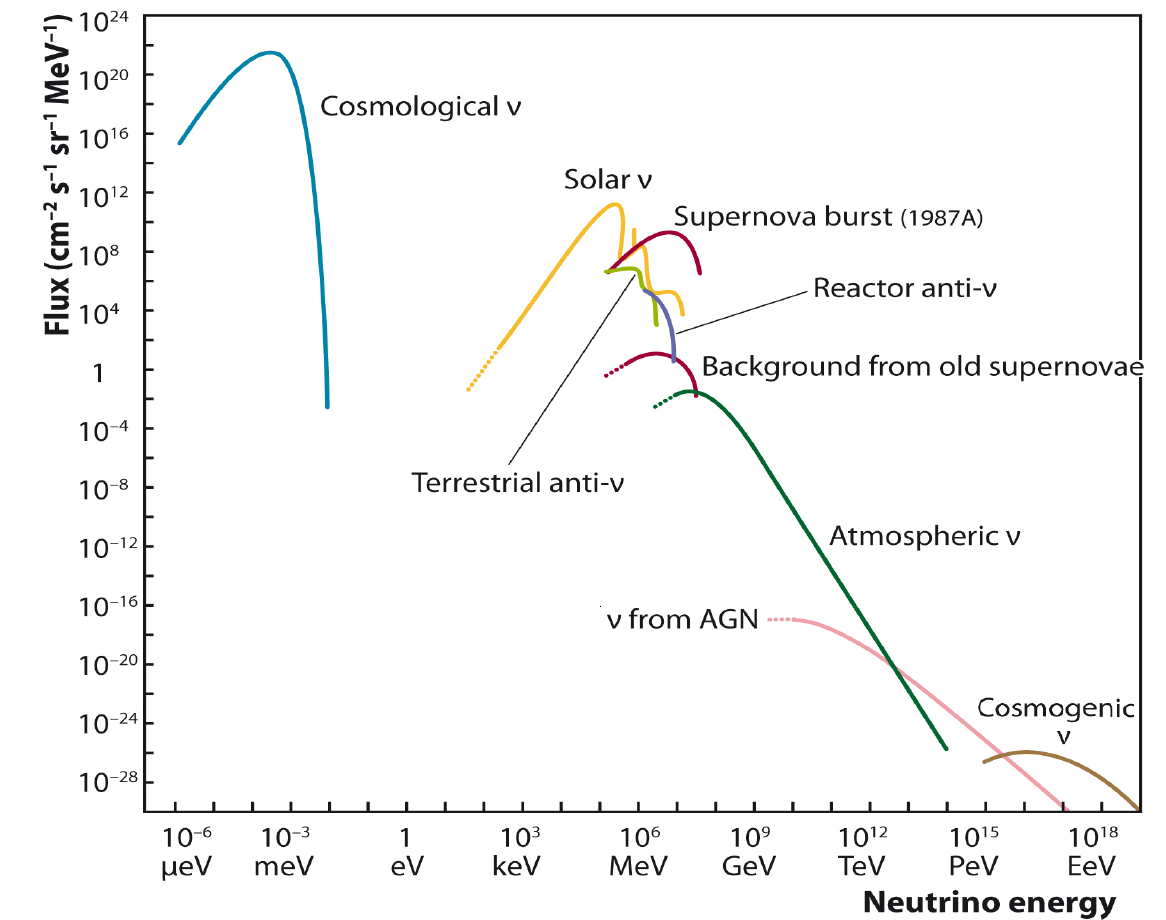
\includegraphics[width=0.7\textwidth]{chapter3/img/neutrinospectrum.png}
\caption{Plot illustrating several neutrino sources that cover a huge range of energy. Illustration from Ref. \cite{Katz:2011ke}.}
\label{fig:neutrinospectrumall}
\end{figure}

Cosmic rays are deflected in magnetic fields and therefore, their arrival direction at Earth does not hold much pointing information (Figure \ref{fig:sourceinfo}, left). Light ranging from radio to gamma rays in the electromagnetic spectrum is of crucial importance in astrophysics but has its limitations: photons can be absorbed by interstellar medium, or are trapped in opaque sources. At higher energies ($\approx 10^{14}$ eV), photons interact with the CMB and produce electron-positron pairs ($\gamma + \gamma \rightarrow e^+ + e^-$). Unless the sources are close by, no photons are capable of reaching Earth (see Figure \ref{fig:opaquephotons}, right). Neutrinos escape from the sources more easily and are not deflected by magnetic fields, making them key messengers in identifying cosmic ray accelerators. As mentioned in Section \ref{sec:airshowers}, neutrinos are also produced in air showers. In the following, we will go over the different types of neutrinos that are detectable on Earth.


\begin{figure}[t]
\centering
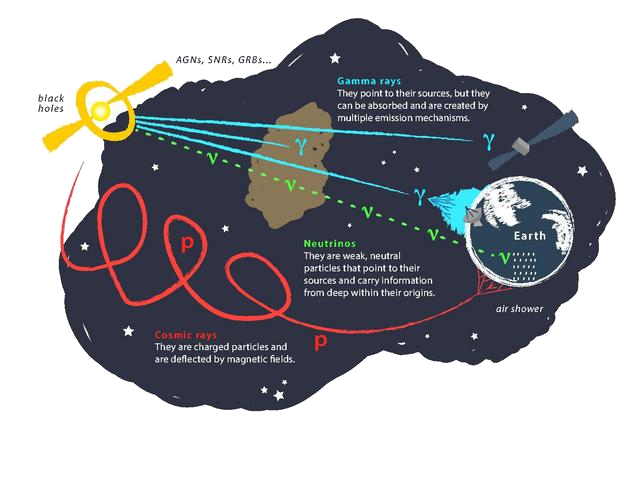
\includegraphics[width=0.6\textwidth]{chapter3/img/sourceinformation_3.jpg}
\caption{Artist impression of the path that several types of particles travel before reaching Earth.}
\label{fig:sourceinfo}
\end{figure}

\begin{figure}[t]
\centering
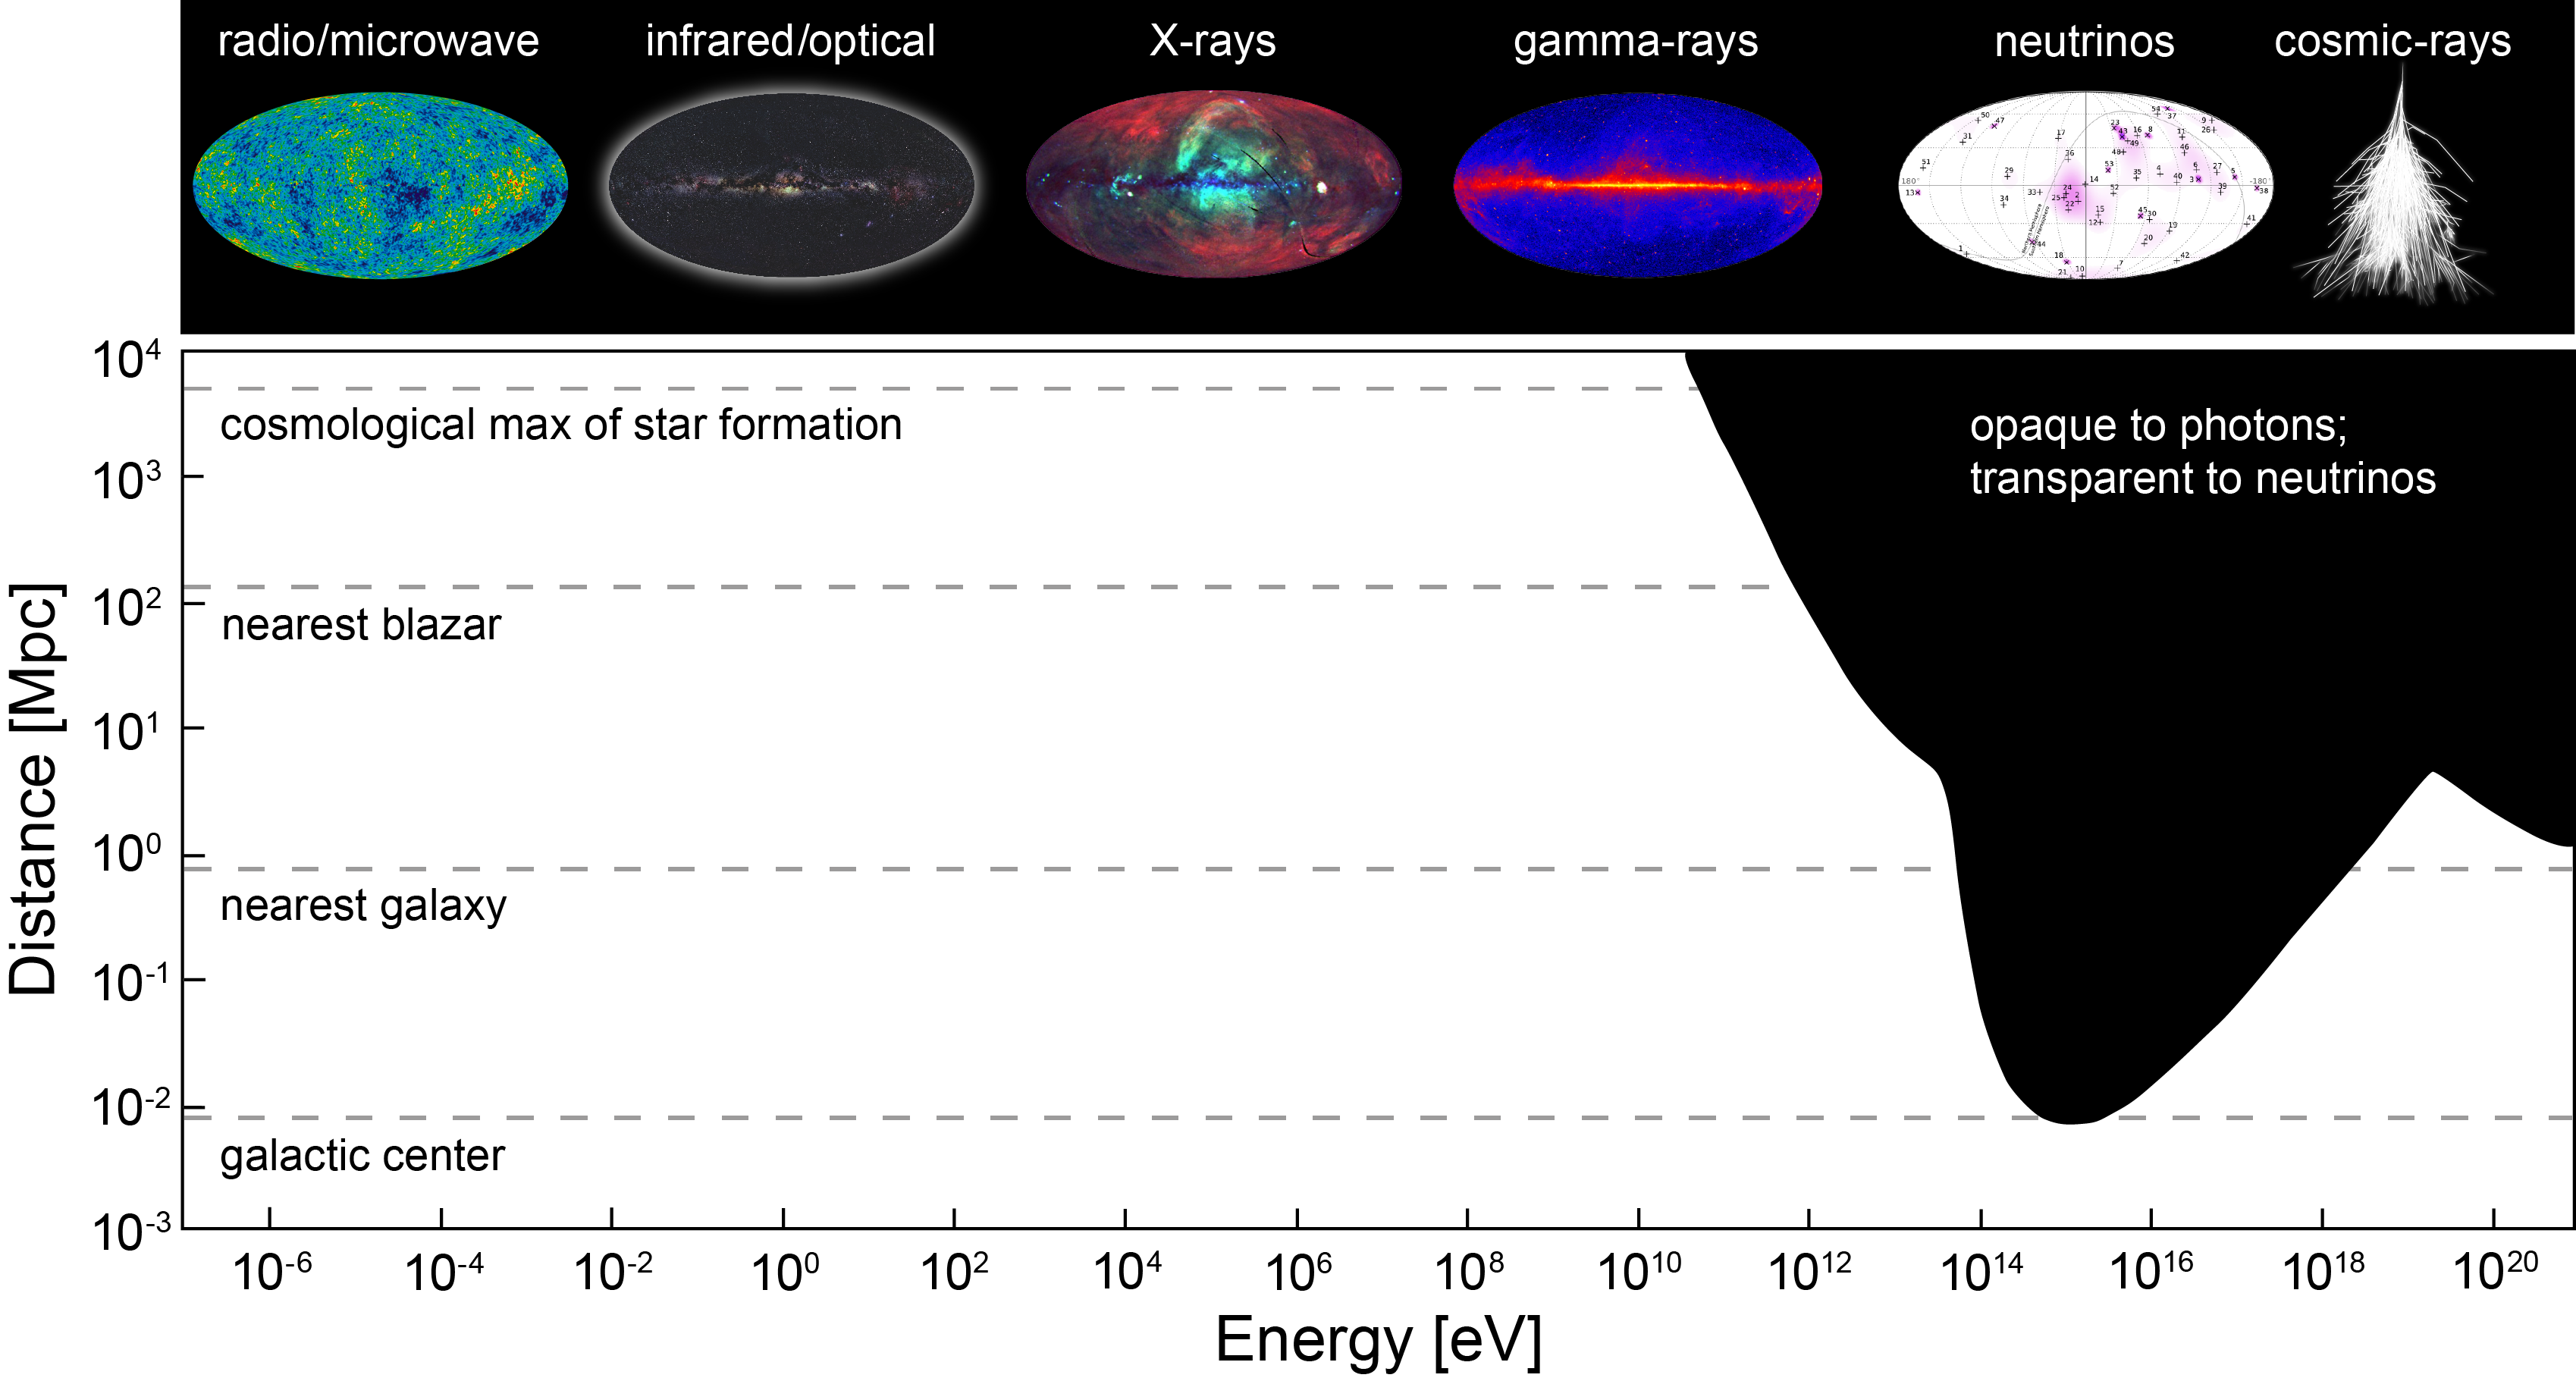
\includegraphics[width=0.6\textwidth]{chapter3/img/opaque-to-photons.png}
\caption{Illustration of the visibility of sources in function of their distance and the photon energy. The dip in the photon visibility comes from the pair production peak when photons interact with the CMB. Both illustrations from the IceCube collaboration.}
\label{fig:opaquephotons}
\end{figure}

\subsection{Conventional}
Neutrinos are produced in large abundances in air showers (see Section \ref{sec:airshowers}; Eq. \ref{eq:hadronic} and \ref{eq:muonic}). The neutrinos that are produced with low to high energies ($\approx$MeV to PeV range) are called \textit{atmospheric} or \textit{conventional} neutrinos. They are primarily produced in pion or kaon decay. Due to helicity effects, pion and kaon decay to electrons/electron neutrinos is strongly suppressed compared to decays into muons/muon neutrinos. As a result, the ratio of electron neutrinos to muon neutrinos is about 2

\begin{equation}
\frac{N\left( \nu_\mu + \bar{\nu}_\mu\right) }{N\left(\nu_e + \bar{\nu}_e\right)} \approx 2,
\end{equation}
which should be clear when we look at the example of pion decay where the muon decays as well

\begin{align}
\pi^+ &\rightarrow \mu^+ + \nu_\mu \nonumber \\
& \rightarrow e^+ + \nu_e + \bar{\nu}_\mu + \nu_\mu.
\end{align}
The most referred to calculations for the atmospherical neutrino flux were done by Honda et al. \cite{Honda:2006qj}.
\begin{figure}[t]
\centering
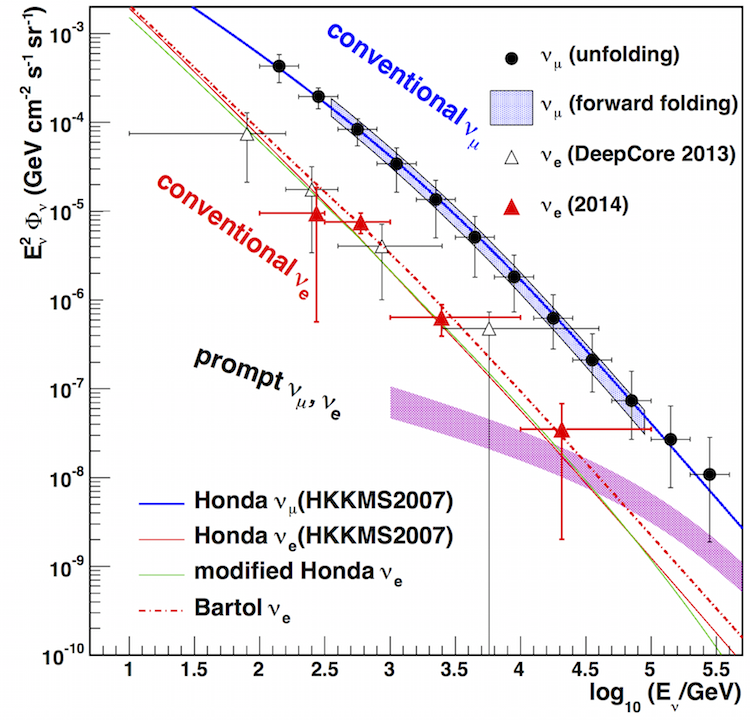
\includegraphics[width=0.39\textwidth]{chapter3/img/neutrinospectrum2.png}
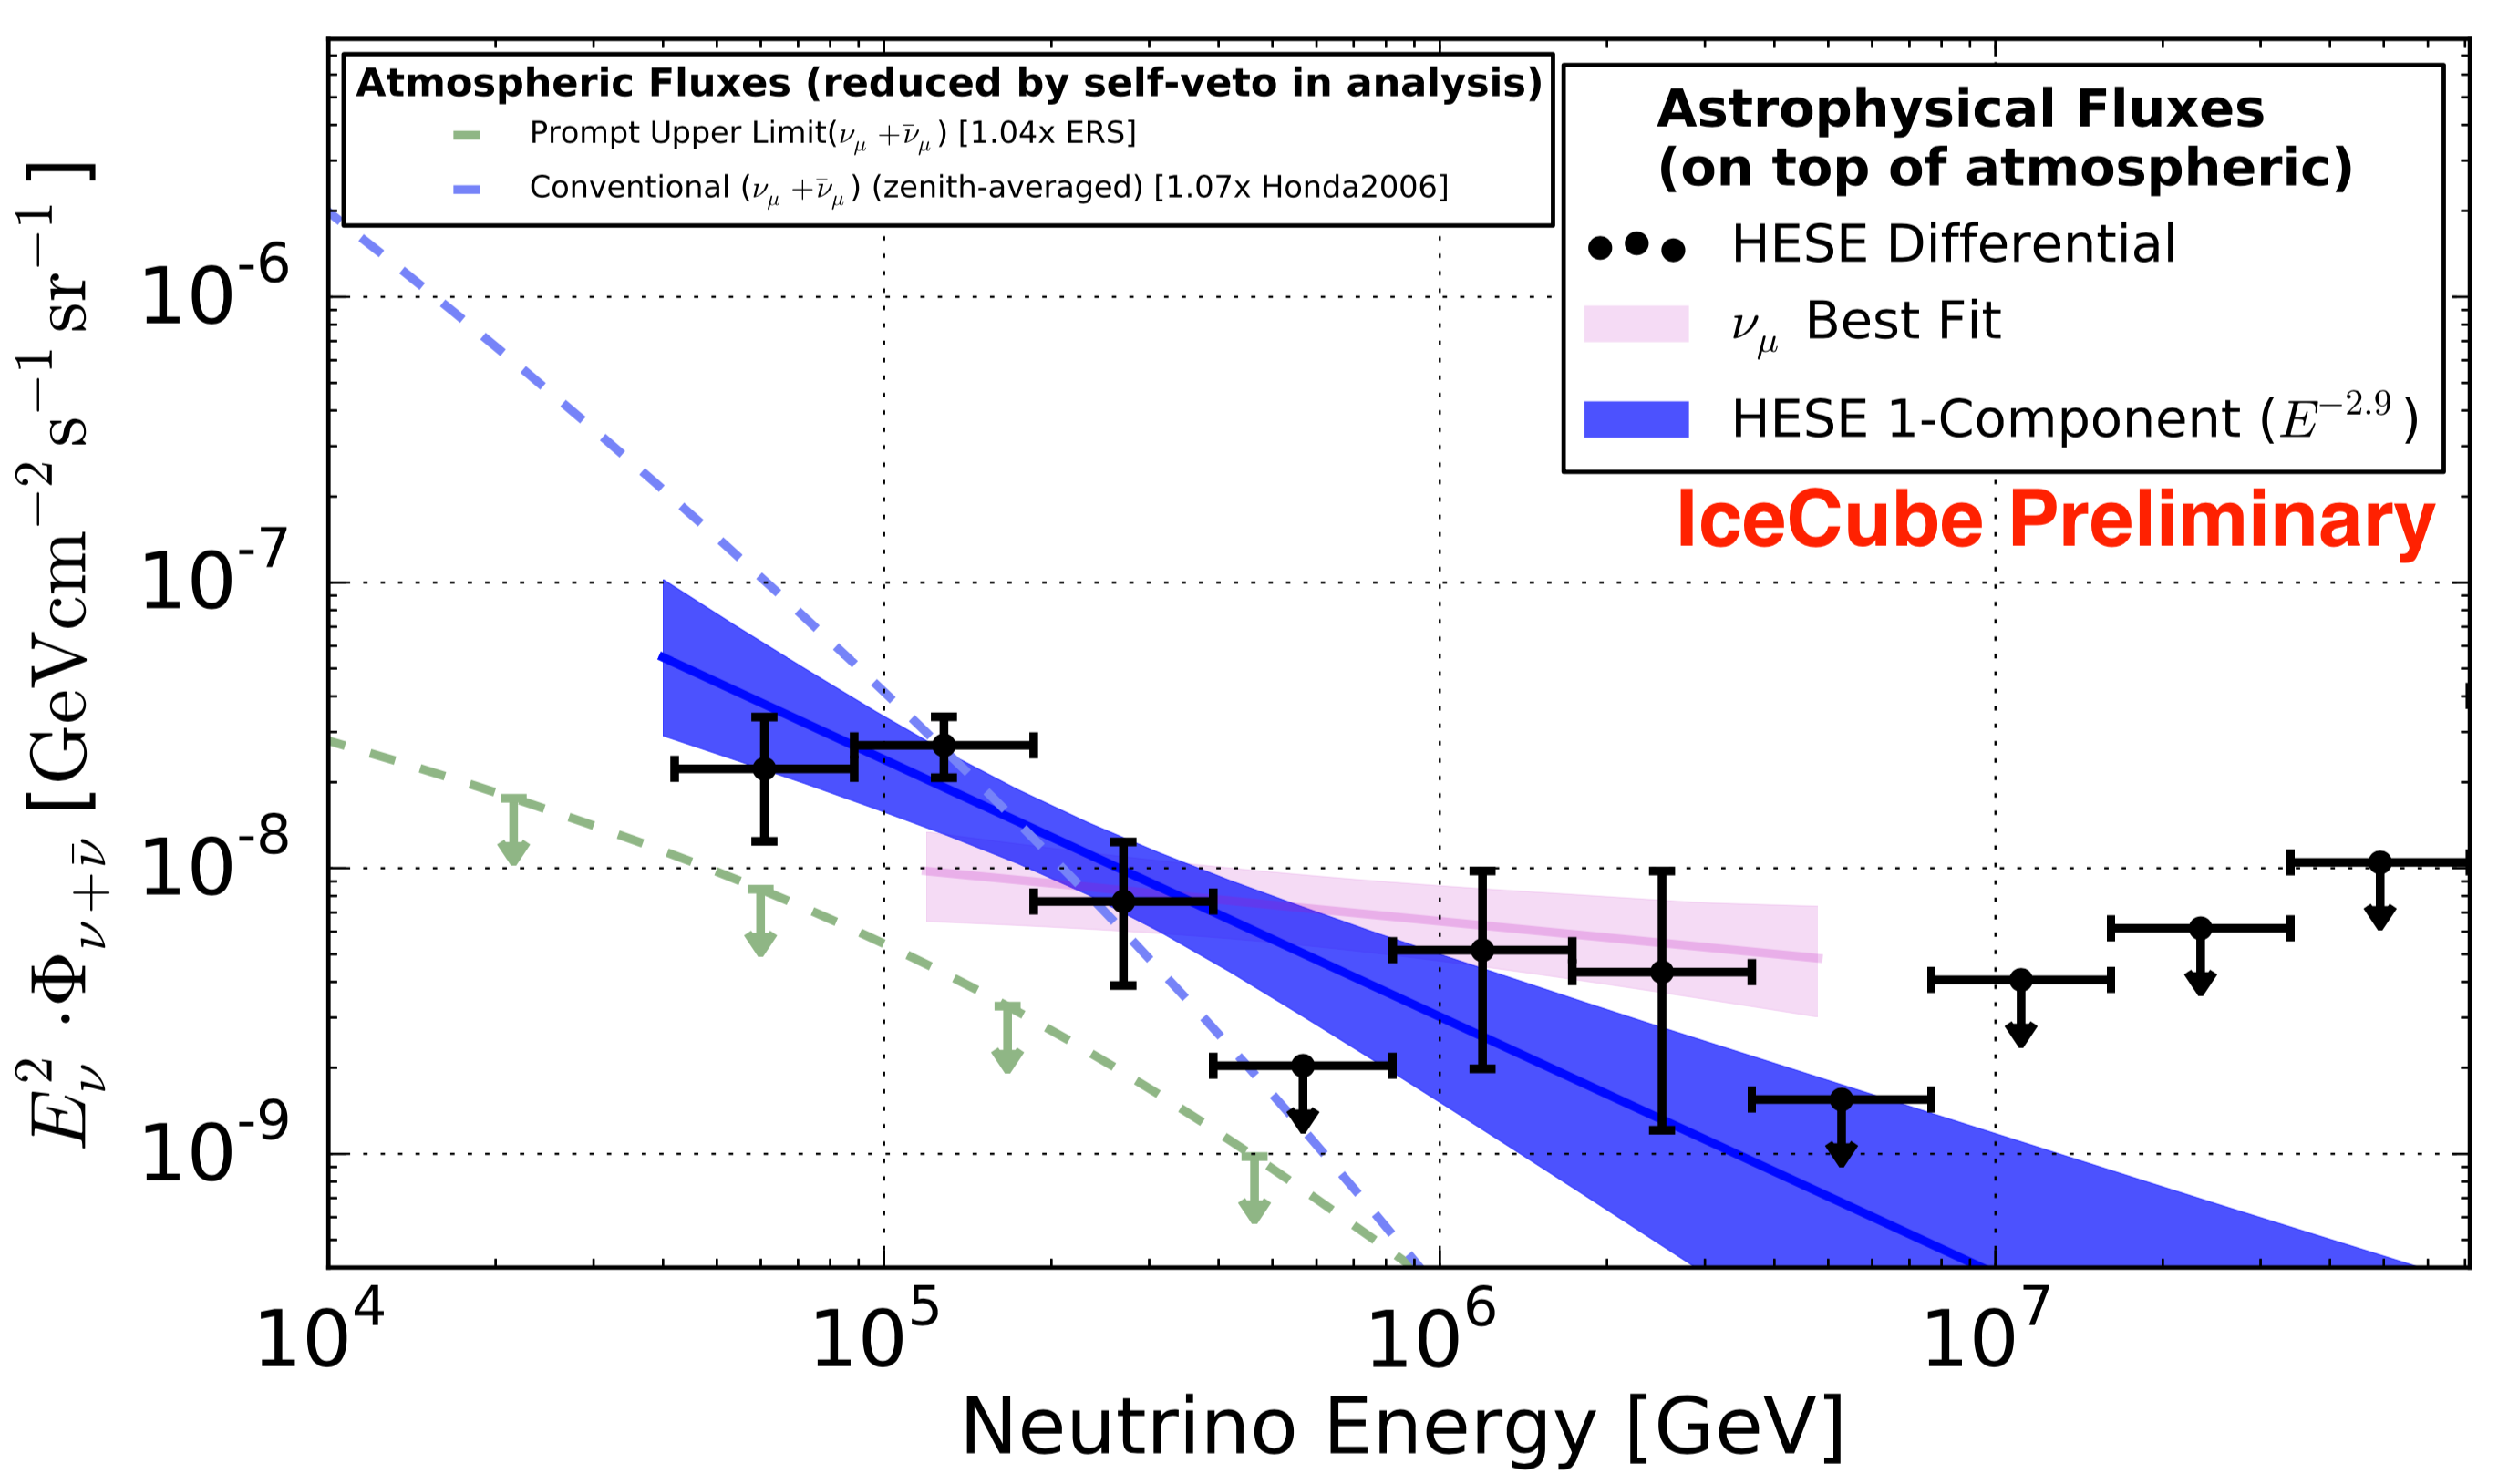
\includegraphics[width=0.6\textwidth]{chapter3/img/astroflux.png}
\caption{\textit{Left}: Measurement from the IceCube collaboration showing the difference in $\nu_e$ and $\nu_\mu$ flux. \textit{Right}: Measured differential astrophysical flux using contained events (points) and a fit to that data (blue line and band), compared with the best fit obtained from through-going $\nu_\mu$ (pink line and band). From Ref. \cite{Aartsen:2017mau}.}.
\label{fig:neutrinospectrum2}
\end{figure}

\subsection{Prompt}
Charmed mesons, also called D mesons, are the lightest particles that contain charm quarks\footnote{$D^0: c\bar{u}, \bar{D}^0: u\bar{c}, D^+: c\bar{d}, D^-: d\bar{c}$}. Hints of charm particles were first seen in cosmic rays in 1971 by Niu et al. \cite{doi:10.1143/PTP.46.1644}. The production of these particles is strongly suppressed, but is expected to exhibit a harder spectrum than conventional neutrinos do. These mesons have short lifetimes (hence the name: prompt) and decay into neutrinos independent of their energy and arrival direction. Therefore, their energy spectrum is expected to follow that of primary cosmic rays. Their contribution at higher energies can be non-negligible or even become dominant. To this date, it has not been possible to observe this prompt component, but it remains an interesting signal in diffuse neutrino searches and could contribute significantly to background expectations, usually in analyses looking for high-energy neutrinos. The most referred to calculations for the prompt neutrino flux were done by Endberg et al. \cite{Enberg:2008te}.
\subsection{Astrophysical}
\label{subsec:astro}
Astrophysical neutrinos are expected to be created when cosmic rays interact close to their interaction sites. Because they are neutral and are unlikely to be absorbed, astrophysical neutrinos are expected to reveal more information about these sources. To first order, these neutrinos would follow the spectrum of cosmic rays at their production. As indicated in Section \ref{para:power}, this is equal to an $E^{-2}$ powerlaw spectrum from Fermi shock acceleration. The majority of these neutrinos are expected to arise from decays from pions that were created in these cosmic-ray interactions ($\pi \rightarrow \mu + \nu_\mu$) followed by the muon decay ($\mu \rightarrow e + \nu_e + \nu_\mu$). The resulting flavor ratio fraction is $\nu_e: \nu_\mu: \nu_\tau = 1:2:0$ at the source. Neutrino oscillations\footnote{Explained in Section \ref{subsec:particlemixing}.} across cosmological distances give an expected $\nu_e: \nu_\mu: \nu_\tau = 1:1:1$ expectation at Earth. Given the tension between different analyses, as can be seen in Figure \ref{fig:neutrinospectrum2}, it is still unclear if the spectrum at high energies can be described with a single power law or something more complex.

The spectrum is expected to follow a harder spectrum compared to the conventional and prompt neutrinos and dominate at the highest energies.\\

\noindent Recently, a collaborative effort of IceCube, Fermi-LAT, MAGIC and others observed a coincidence of high-energy neutrinos and a blazar, making them very good candidates of sources of astrophysical neutrinos \cite{IceCube:2018dnn}.

\subsection{Other neutrino sources}
The abovementioned neutrino sources are most important for high-energy neutrino research. Other, more abundant sources such as cosmological, solar, terrestrial and reactor neutrinos, play less of a role in kilometer scaled detectors such as the IceCube detector (see Chapter \ref{ch:icecube}). Supernova and GZK neutrinos have not yet been observed but are a part of the experiment's search strategies and therefore briefly explained below.

%\subsubsection{Cosmological}
%Similar to the photons from the CMB, neutrinos would have been able to decouple from matter only seconds after the Big Bang. Due to the expansion of the universe, the temperature of the neutrinos has dropped to $\approx 1.95$ K due to redshift. At these energies, direct detection is near to impossible. They have no measurable effect in large-scale neutrino detectors.
 
%Mooie uitleg van redshift: https://www.forbes.com/sites/startswithabang/2016/09/09/cosmic-neutrinos-detected-confirming-the-big-bangs-last-great-prediction/
%\subsubsection{Solar}
%Nuclear fusion in the Sun is responsible for the production of electron neutrinos and is the largest contribution of neutrinos that can be detected on Earth. 86\% of neutrinos are produced by the proton-proton reaction

%\begin{equation}
%p + p \rightarrow d + e^+ + \nu_e.
%\end{equation}
%The remaining part is produced by reactions that involve more heavy particles. Having energies $<$ 20 MeV, these neutrinos have no measurable effect in neutrino telescopes.
%\subsubsection{Terrestrial neutrinos}
%Radioactive decays from $\ce{^{40}K}$, $\ce{^{232}Th}$ and $\ce{^{238}U}$ account for almost all geoneutrinos. The reactions give rise to neutrinos from beta decay \cite{Wan:2016nhe}

%\begin{alignat}{2}
%\ce{^{40}_{19}K} + e^- &\rightarrow \ce{^{40}_{18}Ar} + \nu_e \ \ &&+1.505 \textrm{ MeV,}\\
%\ce{^{40}_{19}K} &\rightarrow \ce{^{40}_{20}Ca} +e^- + \bar{\nu}_e \ \ &&+1.311 \textrm{ MeV,}\\
%\ce{^{232}_{90}Th} &\rightarrow \ce{^{208}_{82}Pb} +6\alpha + 4e^- +4\bar{\nu}_e\ \ &&+42.652 \textrm{ MeV,} \\
%\ce{^{235}_{92}U} &\rightarrow \ce{^{207}_{82}Pb} + 7\alpha + 4e^- + 4\bar{\nu}_e \ \ &&+46.402 \textrm{ MeV,}\\
%\ce{^{238}_{92}U} &\rightarrow \ce{^{206}_{82}Pb} +8\alpha +6e^- + 6\bar{\nu}e \ \ &&+51.698 \textrm{ MeV.}
%\end{alignat}
%The maximal energies of these neutrinos are again too low to give a contribution to neutrino telescopes.
%\subsubsection{Reactor neutrinos}
%Nuclear reactors harness energy from the splitting (fission) of heavy nuclei into lighter fission products. These neutron-rich daughter particles undergo beta decays ($n \rightarrow p+e^-+\bar{\nu}_e$). Reactor neutrinos are therefore always antineutrinos. The energy spectrum reaches a maximum around 10 MeV, making them again invisible for neutrino telescopes. 

\subsubsection{Supernova neutrinos}
The core collapse of stars where electrons and protons are compressed into neutrons as described in Section \ref{subsubsec:supernovae} dissipates most of its energy in the production of neutrinos ($e^- + p^+ \rightarrow n + \nu_e$) \cite{Scholberg:2012id}. Since the IceCube detector is designed to detect neutrinos with an energy greater than 100 GeV, supernova neutrinos with an energy of a couple of MeV are only visible to the detector due to a collective raise of individual hits of the equipment. The sensitivity ranges from 20 standard deviations at the galactic edge (30 kpc) and 6 standard deviations at the Large Magellanic Cloud (50 kpc) \cite{Kopke:2011xb}.

\subsubsection{GZK neutrinos}
The GZK-effect was introduced in Section \ref{subsec:extragalactic} where it was explained how high-energy cosmic rays interact with the CMB. The pions that are produced in this process can decay to neutrinos. These neutrinos are expected to have an energy above $\sim 10$ PeV. To this date, no neutrino events with an unquestionable GZK origin have been observed \cite{Ishihara:2017szg}. There are, however, ongoing experiments trying to measure the flux of these extremely energetic neutrinos (see Section \ref{subsub:radio}).





%\section{Cosmic ray and neutrino detectors}
%\label{sec:detectors}
%\textcolor{red}{Doen of niet? Kan een interessante overgang geven naar hoofdstuk 5 en IceCube meer introduceren... Kan ook teveel info zijn. In 10-tal zinnen?}

%Heel kort: pg 5 Gaisser boek. Zo IC introduceren.

%VERITAS, HESS, MAGIC, HAWC, PA, TA, Super-K, Antares, IceCube

%The IceCube Collaboration instead tested the principle using neutrinos. Neutrinos interact with matter through the weak force — one of the four fundamental forces of nature. The influence of the weak force is limited to minute distances. As a result, interactions between neutrinos and matter are extremely improbable, and a neutrino can easily traverse the entire Earth unimpeded. This poses a challenge for physicists trying to study these elusive particles, because almost every neutrino will simply pass through any detector completely unnoticed.
